% \iffalse meta-comment
%<*internal|ijdc9|ijdc14|idcc|base>
\def\Version{2020/01/15 v2.0}
%</internal|ijdc9|ijdc14|idcc|base>
%<*internal>
\iffalse
%</internal>
%<*readme>
# The dccpaper bundle: LaTeX classes for submissions to IJDC and IDCC

The dccpaper bundle consists of three very similar classes.

ijdc-v14.cls corresponds to the template used by the
[International Journal of Digital Curation], beginning with volume 14.

ijdc-v9.cls corresponds to the template used by the
[International Journal of Digital Curation] for volumes 9 to 13 inclusive.

idcc.cls corresponds to the template used for the
[International Digital Curation Conference], beginning with IDCC15.

As the classes are so similar, their common features are abstracted out
into dccpaper-base.sty; please do not attempt to use this package
independently of the above classes.

The classes are suitable for submissions to the respective review
boards, but can also be used to produce the final camera-ready papers.

[International Journal of Digital Curation]: http://www.ijdc.net/index.php/ijdc
[International Digital Curation Conference]: http://www.dcc.ac.uk/events/international-digital-curation-conference-idcc

%</readme>
%<ijdc9|ijdc14|idcc|base>\NeedsTeXFormat{LaTeX2e}[1999/12/01]
%<*ijdc9>
\ProvidesClass{ijdc-v9}
    [\Version\space Class for submissions to the International Journal of Digital Curation, volumes 9--13 inclusive.]
%</ijdc9>
%<*ijdc14>
\ProvidesClass{ijdc-v14}
    [\Version\space Class for submissions to the International Journal of Digital Curation, volume 14 onwards.]
%</ijdc14>
%<*idcc>
\ProvidesClass{idcc}
    [\Version\space Class for submissions to the International Digital Curation Conference.]
%</idcc>
%<*base>
\ProvidesPackage{dccpaper-base}
    [\Version\space Common class code for IJDC and IDCC papers.]
%</base>
%<*biblatex|apacite>
@book{apa6ed,
  author = {{American Psychological Association}},
  shortauthor = {{APA}},
  publisher = {Author},
%<biblatex>  date = {2010},
%<apacite>  year = {2010},
  title = {Publication manual of the {American} {Psychological} {Association}},
  edition = {6},
%<biblatex>  location = {Washington, DC}
%<apacite>  address = {Washington, DC}
}

@book{borgman2007sda,
  author = {Borgman, C. L.},
%<biblatex>  date = {2007},
%<apacite>  year = {2007},
%<biblatex>  title = {Scholarship in the digital age},
%<biblatex>  subtitle = {Information, infrastructure, and the {Internet}},
%<apacite>  title = {Scholarship in the digital age: Information, infrastructure, and the {Internet}},
%<biblatex>  location = {Cambridge, MA},
%<apacite>  address = {Cambridge, MA},
  publisher = {MIT Press}
}

@inbook{borgman.etal2006bdl,
  author = {Borgman, C. L. and Wallis, J. C. and Enyedy, N.},
%<biblatex>  date = {2006},
%<apacite>  year = {2006},
%<biblatex>  title = {Building digital libraries for scientific data},
%<biblatex>  subtitle = {An exploratory study of data practices in habitat ecology},
%<apacite>  title = {Building digital libraries for scientific data: An exploratory study of data practices in habitat ecology},
  editor = {J. Gonzalo and C. Thanos and M. F. Verdejo and R. C. Carrasco},
%<biblatex>  booktitle = {{Lecture} {Notes} in {Computer} {Science}},
%<biblatex>  booksubtitle = {Vol. 4172. {Research} and {Advanced} {Technology} for {Digital} {Libraries}},
%<apacite>  booktitle = {{Lecture} {Notes} in {Computer} {Science:} {Vol.} 4172. {Research} and {Advanced} {Technology} for {Digital} {Libraries}},
  pages = {170--183},
  doi = {10.1007/11863878_15}
}

%<biblatex>@report{ccsds2012oais,
%<apacite>@techreport{ccsds2012oais,
  author = {{Consultative Committee for Space Data Systems}},
  shortauthor = {{CCSDS}},
%<biblatex>  date = {2012},
%<apacite>  year = {2012},
  title = {Reference model for an {Open} {Archival} {Information} {System} {(OAIS)}},
  type = {Magenta Book},
  number = {CCSDS 650.0-M-2},
  url = {http://public.ccsds.org/publications/archive/650x0m2.pdf}
}

%<biblatex>@report{dcc2005dcp,
%<apacite>@techreport{dcc2005dcp,
  author = {{Digital Curation Centre}},
%<biblatex>  date = {2005},
%<apacite>  year = {2005},
%<biblatex>  title = {Digital curation and preservation},
%<biblatex>  subtitle = {Defining the research agenda for the next decade},
%<apacite>  title = {Digital curation and preservation: Defining the research agenda for the next decade},
%<apacite>  type = {\bibnotype},
%<biblatex>  note = {Report of the Warwick Workshop, November 7–8, 2005},
%<apacite>  howpublished = {Report of the Warwick Workshop, November 7–8, 2005},
  url = {http://www.dcc.ac.uk/webfm_send/346}
}

@article{esanu.etal2004sar,
  author = {Esanu, J. and Davidson, J. and Ross, S. and Anderson, W.},
%<biblatex>  date = {2004},
%<apacite>  year = {2004},
%<biblatex>  title = {Selection, appraisal, and retention of digital scientific data},
%<biblatex>  subtitle = {Highlights of an {ERPANET\slash CODATA} workshop},
%<apacite>  title = {Selection, appraisal, and retention of digital scientific data: Highlights of an {ERPANET\slash CODATA} workshop},
%<biblatex>  journaltitle = {Data Science Journal},
%<apacite>  journal = {Data Science Journal},
  volume = {3},
  pages = {227--232},
  url = {http://www.jstage.jst.go.jp/browse/dsj}
}

@article{mazairac.beetzIPboq,
  author = {Mazairac, W. and Beetz, J.},
%<biblatex>  pubstate = {inpress},
%<apacite>  year = {\BIP},
%<biblatex>  title = {{BIMQL}},
%<biblatex>  subtitle = {An Open Query Language for Building Information Models},
%<apacite>  title = {{BIMQL}: An Open Query Language for Building Information Models},
%<biblatex>  journaltitle = {Advanced Engineering Informatics},
%<apacite>  journal = {Advanced Engineering Informatics},
  doi = {10.1016/j.aei.2013.06.001}
}

%<biblatex>@report{nsf2003rse,
%<apacite>@techreport{nsf2003rse,
  author = {{National Science Foundation, Blue-Ribbon Advisory Panel on Cyberinfrastructure}},
%<biblatex>  date = {2003},
%<apacite>  year = {2003},
  title = {Revolutionizing science and engineering through cyberinfrastructure},
%<apacite>  type = {\bibnotype},
  url = {http://www.nsf.gov/publications/pub_summ.jsp?ods_key=cise051203}
}

@article{rinaldo.etal2011rsc,
  author = {Rinaldo, C. and Warnement, J. and Baione, T. and Kalfatovic, M. R. and Fraser, S.},
%<biblatex>  date = {2011-07},
%<apacite>  year = {2011},
%<apacite>  month = jul,
  title = {Retooling special collections digitisation in the age of mass scanning},
%<biblatex>  journaltitle = {Ariadne},
%<apacite>  journal = {Ariadne},
  volume = {67},
  url = {http://www.ariadne.ac.uk/issue67/rinaldo-et-al/}
}

@unpublished{santini2004sas,
  author = {Santini, M.},
%<biblatex>  date = {2004},
%<apacite>  year = {2004},
  title = {A shallow approach to syntactic feature extraction for genre classification},
  howpublished = {Paper presented at the Seventh Annual Colloquium for the UK Special Interest Group for Computational Linguistics, Birmingham, UK},
  url = {ftp://ftp.itri.bton.ac.uk/reports/ITRI-04-02.pdf}
}

%<biblatex>@report{santini2004saa,
%<apacite>@techreport{santini2004saa,
  author = {Santini, M.},
%<biblatex>  date = {2004},
%<apacite>  year = {2004},
  title = {State-of-the-art on automatic genre identification},
  type = {Technical Report},
  number = {ITRI-04-03},
  institution = {Information Technology Research Institute},
  url = {ftp://ftp.itri.bton.ac.uk/reports/ITRI-04-03.pdf}
}

@article{smith.etal2003das,
  author = {Smith, M. and Barton, M. and Bass, M. and Branschofsky, M. and McClellan, G. and Stuve, D. and Walker, J. H.},
%<biblatex>  date = {2003},
%<apacite>  year = {2003},
%<biblatex>  title = {{DSpace}},
%<biblatex>  subtitle = {An open source dynamic digital repository},
%<apacite>  title = {{DSpace}: An open source dynamic digital repository},
%<biblatex>  journaltitle = {D-Lib Magazine},
%<apacite>  journal = {D-Lib Magazine},
  volume = {9},
  number = {1},
  doi = {10.1045/january2003-smith}
}

%<biblatex>@data{waterton.etal2013ual,
%<apacite>@misc{waterton.etal2013ual,
  author = {Waterton, C. and Watson, N. and Norton, L.},
  title = {Understanding and Acting in {Loweswater}, 2007–2010},
%<biblatex>  entrysubtype = {Data set},
%<apacite>  type = {Data set},
%<biblatex>  date = {2013},
%<apacite>  year = {2013},
  publisher = {UK Data Archive},
%<biblatex>  location = {Colchester, UK},
%<apacite>  address = {Colchester, UK},
  doi = {10.5255/UKDA-SN-7359-1}
}

@book{witten.frank2005dmp,
  author = {Witten, I. H. and Frank, E.},
%<biblatex>  date = {2005},
%<apacite>  year = {2005},
%<biblatex>  title = {Data mining},
%<biblatex>  subtitle = {Practical machine learning tools and techniques},
%<apacite>  title = {Data mining: Practical machine learning tools and techniques},
  edition = {2},
%<biblatex>  location = {San Francisco, CA},
%<apacite>  address = {San Francisco, CA},
  publisher = {Morgan Kaufmann}
}
%</biblatex|apacite>
%<*internal>
\fi
\def\nameofplainTeX{plain}
\ifx\fmtname\nameofplainTeX\else
  \expandafter\begingroup
\fi
%</internal>
%<*install>
\input docstrip.tex
\keepsilent
\askforoverwritefalse
\preamble

----------------------------------------------------------------
The dccpaper bundle: Classes for submissions to IJDC and IDCC
Author:  Alex Ball
E-mail:  a.ball@ukoln.ac.uk
License: Released under the LaTeX Project Public License v1.3c or later
See:     http://www.latex-project.org/lppl.txt
----------------------------------------------------------------

\endpreamble
\postamble

Copyright (C) 2020 Digital Curation Centre, University of Edinburgh
<info@dcc.ac.uk>
\endpostamble

\usedir{tex/latex/dccpaper}
\generate{
  \file{ijdc-v9.cls}{\from{\jobname.dtx}{ijdc9}}
  \file{ijdc-v14.cls}{\from{\jobname.dtx}{ijdc14}}
  \file{idcc.cls}{\from{\jobname.dtx}{idcc}}
  \file{dccpaper-base.sty}{\from{\jobname.dtx}{base}}
}
%</install>
%<install>\endbatchfile
%<*internal>
\usedir{source/latex/dccpaper}
\generate{
  \file{\jobname.ins}{\from{\jobname.dtx}{install}}
}
\nopreamble\nopostamble
\usedir{doc/latex/dccpaper}
\generate{
  \file{README.md}{\from{\jobname.dtx}{readme}}
  \file{dccpaper-biblatex.bib}{\from{\jobname.dtx}{biblatex}}
  \file{dccpaper-apacite.bib}{\from{\jobname.dtx}{apacite}}
}
\ifx\fmtname\nameofplainTeX
  \expandafter\endbatchfile
\else
  \expandafter\endgroup
\fi
%</internal>
%<*driver>
\ProvidesFile{dccpaper.dtx}
    [\Version\ Classes for submissions to IJDC and IDCC]
\documentclass{ijdc-v14}
\let\DccpaperMaketitle=\maketitle

% For typesetting the documentation generally
\usepackage{doc}
\usepackage{enumitem}
\usepackage{listings}
\colorlet{Command}{red!75!black}
\colorlet{Environment}{blue!75!black}
\colorlet{Option}{violet}
\colorlet{Value}{olive!75!black}
\lstloadlanguages{[LaTeX]TeX}
\lstset
  { columns=fullflexible
  , basicstyle=\ttfamily
  , language={[LaTeX]TeX}
  , texcsstyle=*\color{Command}
  , moretexcs=
    { affil
    , conference
    , correspondence
    , submitted
    , received
    , revised
    , accepted
    , subno
    , volume
    , issue
    , maketitle
    , sisetup
    , toprule
    , cmidrule
    , midrule
    , bottomrule
    , DeclareLanguageMapping
    , printbibliography
    , addbibresource
    , subsection
    , subparagraph
    }
  , moredelim=**[s][\color{Option}]{[}{]}
  , moredelim=**[s][\color{Environment}]{\{}{\}}
  , mathescape
  }
\newcommand*{\pkg}[1]{\href{http://www.ctan.org/pkg/#1}{\textsf{#1}}}
\newcommand*{\cs}[1]{\textcolor{Command}{\texttt{\textbackslash#1}}}
\newcommand*{\env}[1]{\textcolor{Environment}{\ttfamily #1}}
\newcommand*{\key}[1]{\textcolor{Option}{\ttfamily #1}}
\newcommand*{\val}[1]{\textcolor{Value}{\ttfamily #1}}
\let\myrmfamily=\rmfamily
\renewcommand*{\meta}[1]{\ensuremath{\langle\textrm{\emph{#1}}\rangle}}
\def\brackets#1{%
  \texttt{\textcolor{Environment}{\char`\{}#1\textcolor{Environment}{\char`\}}}}
\def\marg#1{%
  \textcolor{Environment}{\ttfamily\char`\{}\meta{#1}\textcolor{Environment}{\ttfamily\char`\}}}
\def\sqbrackets#1{%
  \texttt{\textcolor{Option}{[}#1\textcolor{Option}{]}}}
\def\oarg#1{%
  \textcolor{Option}{\ttfamily\char`\{}\meta{#1}\textcolor{Option}{\ttfamily\char`\}}}
\makeatletter
\let\PrintMacroName=\@gobble
\let\PrintEnvName=\@gobble
\makeatother
\newenvironment{optionkey}[1]{}{}
\newenvironment{optionvalue}[1]{}{}

% For typesetting the implementation
\usepackage{metalogo}
% This bit inspired by ydoc
\makeatletter
\newwrite\ydocwrite
\def\ydocfname{\jobname.lsttemp}
\def\ydoc@catcodes{%
  \let\do\@makeother
  \dospecials
  \catcode`\\=\active
  \catcode`\^^M=\active
  \catcode`\ =\active
}
\def\macrocode{%
  \begingroup
  \ydoc@catcodes
  \macro@code
}
\def\endmacrocode{}
\begingroup
\endlinechar\m@ne
\@firstofone{%
\catcode`\|=0\relax
\catcode`\(=1\relax
\catcode`\)=2\relax
\catcode`\*=14\relax
\catcode`\{=12\relax
\catcode`\}=12\relax
\catcode`\ =12\relax
\catcode`\%=12\relax
\catcode`\\=\active
\catcode`\^^M=\active
\catcode`\ =\active
}*
|gdef|macro@code#1^^M%    \end{macrocode}(*
|endgroup|expandafter|macro@@code|expandafter(|ydoc@removeline#1|noexpand|lastlinemacro)*
)*
|gdef|ydoc@removeline#1^^M(|noexpand|firstlinemacro)*
|gdef|ydoc@defspecialmacros(*
|def^^M(|noexpand|newlinemacro)*
|def (|noexpand|spacemacro)*
|def\(|noexpand|bslashmacro)*
)*
|gdef|ydoc@defrevspecialmacros(*
|def|newlinemacro(|noexpand^^M)*
|def|spacemacro(|noexpand )*
|def|bslashmacro(|noexpand\)*
)*
|endgroup
\def\macro@@code#1{%
  {\ydoc@defspecialmacros
  \xdef\themacrocode{#1}}%
  \PrintMacroCode
  \end{macrocode}%
}
\def\PrintMacroCode{%
  \begingroup
  \let\firstlinemacro\empty
  \let\lastlinemacro\empty
  \def\newlinemacro{^^J}%
  \let\bslashmacro\bslash
  \let\spacemacro\space
  \immediate\openout\ydocwrite=\ydocfname\relax
  \immediate\write\ydocwrite{\themacrocode}%
  \immediate\closeout\ydocwrite
  \let\input\@input
  \lstinputlisting[firstnumber=last]{\ydocfname}%
  \endgroup
}
\makeatother

\let\maketitle=\DccpaperMaketitle

\usepackage{dcolumn,csquotes}
\usepackage[iso,british]{isodate}
\usepackage[expansion=false]{microtype}
\ifXeTeX\else\DisableLigatures{family=tt*}\fi
\usepackage[tightLists=false]{markdown}
\markdownSetup{rendererPrototypes={%
 link = {#1\footnote{\ifx\empty#4\empty\else#4:
 \fi\url{#3}}}%
}}
\def\T#1{}  % Work around bug where \T1 inserted as control sequence
\usepackage{fnpct}

\ifx\undefined\apacitefalse
  \usepackage[style=apa]{biblatex}
  \addbibresource{dccpaper-biblatex.bib}
  \DeclareLanguageMapping{british}{british-apa}
\else
  \usepackage{apacite}
  \bibliographystyle{apacite}
  \let\textcite=\citeA
  \let\autocite=\cite
\fi

\title[The \textsf{dccpaper} bundle]{The \protect\textsf{dccpaper} bundle: Classes for submissions to IJDC and IDCC}

\author{Alex Ball}
\affil{University of Bath}
\correspondence{Alex Ball, University of Bath, Claverton Down, Bath BA2 7AY. Email: \email{a.j.ball@bath.ac.uk}}

\received{4 July 2013}
\revised{10 December 2013}
\accepted{1 January 2014}

\GetFileInfo{dccpaper-base.sty}

\begin{document}
\maketitle

\begin{abstract}
This is the documentation for the \pkg{dccpaper} bundle, consisting of the following classes:
\begin{itemize}
\item\textsf{ijdc-v14}, which corresponds to the template used by the International Journal of Digital Curation, beginning with volume 14.
\item\textsf{ijdc-v9}, which corresponds to the template used by the International Journal of Digital Curation for volumes 9 and 13 inclusive.
\item\textsf{idcc}, which corresponds to the template used for the International Digital Curation Conference, beginning with IDCC15.
\end{itemize}

The version to which it relates is \fileversion, last revised \printdateTeX{\filedate}.

The code for this bundle is maintained at \url{https://github.com/DigitalCurationCentre/dccpaper}.

Versions of the templates are also available that target Microsoft Word and LibreOffice\slash OpenOffice.org.

Please note that the DOI attached to this document is fake and should not be used for identification purposes.
\end{abstract}

\section{Introduction}

The \LaTeX\ class \textsf{ijdc-v14} produces camera-ready papers and articles suitable for inclusion in the International Journal of Digital Curation, with applicability from volume 14 onwards. This is a minor change to the template used for volumes 9--13, which remains available as \textsf{ijdc-v9}. The similar \textsf{idcc} class can be used for submissions to the International Digital Curation Conference, beginning with the 2015 conference. This document explains how to use these classes.

\section{Dependencies}

Certain aspects of the template design have been implemented using third-party packages, aside from those that are required parts of the \LaTeX\ system. Therefore you should ensure that you have these packages installed on your system before attempting to use the class.

\begin{itemize}
\item\pkg{atbegshi} is used for switching geometry between pages.
\item Tables in your document must be formatted according to the design principles promoted and supported by the \pkg{booktabs} package.
\item\pkg{caption} is used to format the figure and table captions.
\item\pkg{etoolbox} is used behind the scenes for patching commands.
\item\pkg{footmisc} is used to format the footnotes.
\item\pkg{titlesec} is used to format the section headings.
\item\pkg{iftex} is used to test which \TeX\ engine you are using.
If you use Lua\LaTeX\ or \XeLaTeX\, you will also need \pkg{fontspec}.
\end{itemize}

In some cases the class prefers to use packages that are not part of the base installation (but are nevertheless commonly available in \TeX\ distributions), but will fall back to their base equivalents if necessary.

\begin{itemize}
\item
If using the \textsf{ijdc-v14} class or the \textsf{idcc} class for conferences from
2020, the main text font will be the first available out of Baskerville, BaskervilleF
(\pkg{baskervillef}), Baskervaldx (\pkg{baskervaldx}), Baskervald (\pkg{baskervaldadf}),
or the standard Computer Modern/Latin Modern.
The sans-serif font will be the first available out of Lucida Sans, Go Sans
(\pkg{gofonts}) or Helvetica (\pkg{helvet}).
\item
If using the \textsf{ijdc-v9} class or the \textsf{idcc} class for conferences up
to 2019,
\pkg{newtx} will be used if available in place of \pkg{mathptmx}, and
\pkg{tgheros} will be used in place of \pkg{helvet}.
\item
\pkg{xcolor} will be used if available in place of \pkg{color}.
\end{itemize}

For referencing, you are encouraged to use either \pkg{biblatex-apa} (preferred) or \pkg{apacite}.

\section{Loading the Classes}

\subsection{International Journal of Digital Curation}

The class is loaded in the usual way with
\lstinline|\documentclass[$\meta{options}$]{ijdc-v14}|.
The following options are available:

\begin{description}[font=\normalfont\key]
\item[paper]
Use this for research papers.
\item[article]
Use this for general articles if you like, but you do not have to as the class defaults to this state.
\item[editorial]
Use this for an editorial.
\item[preprint]
Use this for a conference preprint.
\end{description}

\subsection{International Digital Curation Conference}

The class is loaded in the usual way with
\lstinline|\documentclass[$\meta{options}$]{idcc}|.
Two types of option are available. The first relates to the conference to which the submission will be made:
\begin{description}[font=\normalfont]
  \item[\key{15}, \key{16}, \key{17}, \key{18}, \key{19}, \key{20}]
  Use this to select the year of the conference, e.g.\@ \key{20} for 2020.
\end{description}

The second relates to the type of submission:
\begin{description}[font=\normalfont\key]
\item[abstract]
Use this for research and practice paper extended abstracts. It is normally the default.
\item[research]
Use this for full research papers.
\item[practice]
Use this for full practice papers. This becomes the default if you select one of the options for the 2015 to 2018 conferences inclusive.
\item[lightning]
Use this for lightning talk proposals.
\item[data]
(Legacy.) Use this for data paper abstracts and full data papers.
\item[poster]
Use this for poster proposals.
\item[demo]
Use this for demonstration proposals.
\item[bof]
(Legacy.) Use this for Birds of a Feather session proposals.
\item[workshop]
Use this for workshop proposals.
\end{description}

\section{Preamble Commands}

The following commands should be given in the preamble to fill out the document metadata.

The following command should be used in all submissions.

\begin{description}
\item[]
\hskip-\labelsep
\lstinline|\title[$\meta{name}$]{$\meta{full version}$}|
\hskip\labelsep
The long version of the title is shown on the cover page of the submission, while the short version appears in the (even page) headers.
\end{description}

The following commands should be given in general articles and IDCC submissions. They should \emph{not} be given in peer-reviewed IJDC papers until after the peer review process is complete.

\begin{description}
\item[]
\hskip-\labelsep
\lstinline|\author{$\meta{name}$}|
\hskip\labelsep
The name of one author. Repeat the command for each additional author.

It is customary in IJDC and IDCC papers to group authors by institution. Within each institution, the authors are ordered by the level of contribution (or alphabetically where this is equal), and the institutional groups are ordered by the level of contribution of the first author in the group (or alphabetically by first author where this is equal). A different convention may be used if appropriate.

\item[]
\hskip-\labelsep
\lstinline|\affil{$\meta{name}$}|
\hskip\labelsep
The affiliation (institution, company) of the immediately preceding author(s). This command may be repeated as necessary.

\item[]
\hskip-\labelsep
\lstinline|\correspondence{$\meta{name, postal address.}$ Email: \email{$\meta{email address}$}}|
\hskip\labelsep
Name, address and email address of the corresponding author. This information appears in the footer of the cover page.
\end{description}

If an IJDC submission is a reworked conference paper (that has not already been formally published), for reasons of transparency the name of the conference should be given.

\begin{description}
\item[]
\hskip-\labelsep
\lstinline|\conference{$\meta{name of conference}$}|
\hskip\labelsep
The conference at which the earlier version of the paper was presented, e.g.\ ‘the 10th International Digital Curation Conference’.
\end{description}

For IDCC papers, authors are invited to record the date on which they made their submission.

\begin{description}
\item[]
\hskip-\labelsep
\lstinline|\submitted{$\meta{date}$}|
\hskip\labelsep
The date on which the initial submission was made to the conference by the authors.
\end{description}

Some additional commands are used by the editorial team when preparing a submission for publication. Though authors would not normally need to use them, here they are for completeness.

\begin{description}
\item[]
\hskip-\labelsep
\lstinline|\received{$\meta{date}$}|
\hskip\labelsep
The date on which the initial submission was received by the editorial team (IJDC papers only).

\item[]
\hskip-\labelsep
\lstinline|\revised{$\meta{date}$}|
\hskip\labelsep
The date on which the latest revision was received by the editorial team.

\item[]
\hskip-\labelsep
\lstinline|\accepted{$\meta{date}$}|
\hskip\labelsep
The date on which the submission was accepted for publication.

\item[]
\hskip-\labelsep
\lstinline|\subno{$\meta{number}$}|
\hskip\labelsep
The submission number allocated by the IJDC Open Journal System.

\item[]
\hskip-\labelsep
\lstinline|\volume{$\meta{number}$}|
\hskip\labelsep
The number of the IJDC volume in which the submission will be published.

\item[]
\hskip-\labelsep
\lstinline|\issue{$\meta{number}$}|
\hskip\labelsep
The number of the IJDC issue in which the submission will be published.

\item[]
\hskip-\labelsep
\lstinline|\date{$\meta{year}$}|
\hskip\labelsep
The year in which the submission will be published.
\end{description}

\newpage
\section{Document Body}

When it comes to writing the body of the submission, the template should allow you to use the usual \LaTeX\ markup without much adaptation. So, for example, for a full paper or an IDCC extended abstract, you would start as in Figure~\ref{fig:start-paper}.

\begin{figure}[ht]
\begin{lstlisting}[frame=single]
\begin{document}
\maketitle

\begin{abstract}
Text of the abstract\dots
\end{abstract}

\section{Introduction}

The text of the introduction starts here\dots
\end{lstlisting}
\caption{Sample code for the beginning of an IJDC submission or IDCC paper.}
\label{fig:start-paper}
\end{figure}

Please note that if submitting a poster, lightning talk or demonstration proposal to the IDCC instead of a paper, you should \emph{not} use the \texttt{abstract} environment. Instead, start with a section headed `Abstract' as in Figure~\ref{fig:start-abstract} (for posters or lightning talks) or Figure~\ref{fig:start-demo} (overleaf, for demonstrations). Further guidance on how to write such submissions is given on the conference website.

If submitting a workshop proposal, please see the second document template in \hyperref[sec:samples]{Appendix~D}.

\begin{figure}[ht]
\begin{lstlisting}[frame=single]
\begin{document}
\maketitle

\section{Abstract}

The text of the proposal starts here\dots
\end{lstlisting}
\caption{Sample code for the beginning of an IDCC proposal.}
\label{fig:start-abstract}
\end{figure}

\begin{figure}[ht]
\begin{lstlisting}[frame=single]
\begin{document}
\maketitle

\begin{description}
\item[Demo Organiser(s):]~\\
Name, position, organization.
\end{description}

\section{Abstract}

The text of the proposal starts here\dots
\end{lstlisting}
\caption{Sample code for the beginning of an IDCC demonstration proposal.}
\label{fig:start-demo}
\end{figure}

\noindent
IJDC and IDCC papers follow the formatting conventions specified by the \textcite{apa6ed}, with a few minor changes. There are some instances where this affects how you write your submission.

\subsection{Headings}

Five levels of heading are defined (\lstinline|\section| down to \lstinline|\subparagraph|) but most authors only need the first one or two levels. \lstinline|\section| and \lstinline|\subsection| headings should be written in title case, that is, with Each Significant Word Given an Initial Capital, while the remaining headers should be written in sentence case as if running text. Do not end your heading names with full stops\slash periods.

\subsection{Quotations}

Quotations should be put in a \texttt{quote} environment, wrapped in inverted commas, with the citation placed in parentheses at the end.

\begin{quote}
‘Cras porttitor dictum lacus. Class aptent taciti sociosqu ad litora torquent per conubia nostra, per inceptos hymenaeos. In consectetuer, diam at volutpat elementum, libero lectus pulvinar sem.’ (Borgman, 2007)
\end{quote}

\subsection{Tables}

\begin{itemize}
\item
Table text should be in the \lstinline|\small| font size.
\item
Tables should not use vertical lines to separate columns, and ideally should not use horizontal lines to separate rows in the body of the table; white space and text alignment should be sufficient. The top and bottom rules should be drawn with \lstinline|\toprule| and \lstinline|\bottomrule| respectively, with other rules drawn with \lstinline|\midrule| or \lstinline|\cmidrule|. See the documentation of the \pkg{booktabs} package for more information.
\item
Text in the body of tables should normally be left-aligned. Numeric data should be aligned at the decimal point among itself but centred with respect to the heading; the \texttt{D} column type from the \pkg{dcolumn} package and the \texttt{S} column type from the \pkg{siunitx} package are particularly useful for this.
\item
Where decked (subdivided) headings are used, there should be a border beneath the upper-level heading (column spanner) indicating to which of the lower-level headings it applies.
\item
Empty cells can either be left blank or represented by an em dash. A blank cell indicates non-applicability, while an em dash signifies that the data was not collected or has been omitted.
\item
Captions should end in a full stop\slash period and appear above the table.
\end{itemize}

Table~\ref{tab:issues} on the following page demonstrates these features. The code used to produce the table is shown in Figure~\ref{fig:table} (the \pkg{dcolumn} package was loaded in the preamble). Note the different relative positions of the table and figure captions.

\begin{table}[p!]
\caption{Papers and articles published in the IJDC in 2008 and 2009.}
\label{tab:issues}
\centering\small
\begin{tabular}{lD..{2.0}D..{2.0}D..{2.1}D..{2.1}}
\toprule
 & \multicolumn{2}{c}{Frequency} & \multicolumn{2}{c}{Percentage} \\
\cmidrule(lr){2-3}\cmidrule(l){4-5}
Issue
 & \multicolumn{1}{c}{Peer-reviewed} & \multicolumn{1}{c}{General}
 & \multicolumn{1}{c}{Peer-reviewed} & \multicolumn{1}{c}{General} \\
\midrule
3(1) &  9 &  7 & 56.3 & 43.8 \\
3(2) &  5 &  7 & 41.7 & 58.3 \\
4(1) & 10 &  4 & 71.4 & 28.6 \\
4(2) &  8 &  6 & 57.1 & 42.9 \\
4(3) &  3 & 15 & 16.7 & 83.3 \\
\bottomrule
\end{tabular}
\end{table}

\begin{figure}[p!]
\begin{lstlisting}[frame=single]
\begin{table}
\caption{Papers and articles published in the IJDC in 2008 and 2009.}
\label{tab:issues}
\centering\small
\begin{tabular}{lD..{2.0}D..{2.0}D..{2.1}D..{2.1}}
\toprule
& \multicolumn{2}{c}{Frequency} & \multicolumn{2}{c}{Percentage} \\
\cmidrule(lr){2-3}\cmidrule(l){4-5}
Issue
& \multicolumn{1}{c}{Peer-reviewed} & \multicolumn{1}{c}{General}
& \multicolumn{1}{c}{Peer-reviewed} & \multicolumn{1}{c}{General} \\
\midrule
3(1) &  9 &  7 & 56.3 & 43.8 \\
3(2) &  5 &  7 & 41.7 & 58.3 \\
4(1) & 10 &  4 & 71.4 & 28.6 \\
4(2) &  8 &  6 & 57.1 & 42.9 \\
4(3) &  3 & 15 & 16.7 & 83.3 \\
\bottomrule
\end{tabular}
\end{table}
\end{lstlisting}
\caption{Code used to typeset Table~\ref{tab:issues}.}
\label{fig:table}
\end{figure}

\subsection{Reference List and Citations}

As mentioned above, you are encouraged to use either \pkg{biblatex-apa} (with \pkg{biblatex}\slash\pkg{biber}) or \pkg{apacite} (with Bib\TeX) to generate your reference list and citations.

\begin{itemize}
\item
To use \pkg{biblatex} for your reference list, add the following to your preamble:
\begin{lstlisting}
\usepackage[style=apa]{biblatex}
\addbibresource{$\meta{bib file}$.bib}
\end{lstlisting}
Prior to the release of \pkg{biblatex-apa} v7.5, you also needed this line:
\begin{lstlisting}
\DeclareLanguageMapping{british}{british-apa}
\end{lstlisting}
Include \lstinline|\printbibliography| at the end of the document to print the list.
\item
To use \pkg{apacite} for your reference list, add the following to your preamble:
\begin{lstlisting}
\usepackage{apacite}
\bibliographystyle{apacite}
\end{lstlisting}
and include \lstinline|\bibliography{$\meta{bib file}$}| at the end of the document.
\end{itemize}

In-text citations are given parenthetically in author–date format. If author forms part of the narrative, as with \textcite{rinaldo.etal2011rsc}, only the date is added in parenthesis, otherwise both author and date are given \autocite{smith.etal2003das}. Where multiple citations are given at once, the order should be the same as in the reference list, i.e.\ alphabetically by author, with co-authored works coming after singly-authored works, then chronologically \autocite{borgman.etal2006bdl, dcc2005dcp, mazairac.beetzIPboq, santini2004sas, santini2004saa, smith.etal2003das, witten.frank2005dmp}. Please consult the documentation of the package you are using for how to achieve this.

Please \textbf{do not cite entire websites} through the reference list mechanism. Instead, provide the title of the website (in English) and the URL in a footnote.\footnote{Digital Curation Centre: \url{http://www.dcc.ac.uk/}} If the title of the website is not clear from the visible pages, the contents of the HTML title element may be used. Other explanatory notes, whether about the body text or cited items, should also be given as footnotes rather than as endnotes or reference list annotations.\footnote{This avoids unnecessary page turning or scrolling.}

Please \textbf{provide digital object identifiers} (DOIs) for referenced items where available.

The data underlying the results presented in the submission should be placed in an appropriate custodial environment and cited \autocite{waterton.etal2013ual}, with the reference placed in the reference list. The \pkg{biblatex-apa} package provides a \texttt{data} entry type which should be used for datasets; the \texttt{entrysubtype} value should be \enquote{\texttt{Data set}} or similar. If using \pkg{apacite}, use the \texttt{misc} entry type with a \texttt{type} value of \enquote{\texttt{Data set}} or similar.

\section{Acknowledgements}

Any acknowledgements should be placed in a section immediately before the references.\nocite{*}

\ifx\undefined\apacitefalse
  \printbibliography
\else
  \bibliography{dccpaper-apacite.bib}
\fi

\newpage
\section{Appendix A: Change History}

\begin{description}
\item[v2.0] 2020-01-15\\
Added new formatting for IJDC volume 14 and IDCC 20.
\item[v1.8.1] 2019-10-07\\
Updated to work with changed \LaTeX\ internals.
\item[v1.8] 2019-03-08\\
Added details of IDCC 2020.
\item[v1.7.1] 2018-05-14\\
Fixed loading of maths fonts. Reverted experimental formatting.
\item[v1.7] 2018-05-01\\
Added details of IDCC 2019, along with new formatting and submission types.
\item[v1.6] 2017-10-20\\
Added details of IDCC 2018. Allowed files to be unpacked by \TeX\ without compiling. Refactored some documentation commands for efficiency.
\item[v1.5] 2016-08-05\\
Added details of IDCC 2017. Slightly refactored code to convert dccpaper-base.tex into a package, dccpaper-base.sty.
\item[v1.4.1] 2015-06-22\\
Fixed bug preventing compilation in DVI mode.
\item[v1.4] 2015-05-22\\
Added details of IDCC 2016. Improved whitespace handling. Fixed bug triggered by \texttt{demo} option. Fixed missing use of \lstinline|\Authfont|. Added missing DOI tweak for \pkg{biblatex-apa}.
\item[v1.3.2] 2015-01-21\\
Removed dependence on user supplying a title. Fixed bug triggered by numbered sections.
\item[v1.3.1] 2014-10-14\\
Fixed typographical error relating to details of IDCC 2015.
\item[v1.3] 2014-08-07\\
Added documentation of \lstinline|\conference| command. Improved display of footnotes, footnote markers and \texttt{itemize}\slash \texttt{enumerate} lists. Fixed a bug in the handling of author information. Fixed and improved how the transition from first to subsequent page geometry is achieved. Updated the details of IDCC 2015.
\item[v1.2] 2014-04-11\\
Added implementation, installation and licence sections to the Appendix of the documentation. Moved the majority of the file postamble information to the README, and synchronized the latter with the GitHub version. Improved the adaptation of \pkg{apacite} referencing to the house style.
\item[v1.1] 2014-03-06\\
Refactored the source for distribution through CTAN, and to allow the addition of the \textsf{idcc} class.
\item[v1.0] 2013-12-18\\
First public release of \textsf{ijdc-v9} class.
\end{description}

\newpage
\section{Appendix B: Implementation}

\lstset
  { aboveskip=1em plus 0.5em minus 0.2em
  , belowskip=1em plus 0.5em minus 0.2em
  , frame=single
  , numbers=left
  , numberstyle=\color{gray}\footnotesize\itshape
  , basicstyle=\footnotesize\ttfamily
  , breaklines=true
  , escapechar=
  }%
\MakeShortVerb{\|}%
\DocInput{\jobname.dtx}

\newpage
\section{Appendix C: Installation}

\begin{markdown*}{hybrid=true}
%</driver>
%<readme>## Installation
%<readme>
%<*driver|readme>
### Managed way

The latest stable release of the dccpaper bundle has been packaged for
TeX Live and MiKTeX. If you are running TeX Live and have `tlmgr`
installed, you can install the bundle simply by running
`tlmgr install dccpaper`. If you are running MiKTeX, you can install the
bundle by running `mpm --install=dccpaper`. Both `tlmgr` and `mpm` have
GUI versions that you might find friendlier.

### Automated way

A makefile is provided which you can use with the Make utility:

  * Running `make source` generates the derived files
      - README.md
      - ijdc-v9.cls
      - idcc.cls
      - dccpaper-base.sty
      - dccpaper-apacite.bib
      - dccpaper-biblatex.bib
  * Running `make` generates the above files and also dccpaper.pdf.
  * Running `make inst` installs the files in the user's TeX tree.
  * Running `make install` installs the files in the local TeX tree.

### Manual way

 1. Run `tex dccpaper.dtx` to generate the source files.
 2. Compile dccpaper.dtx with (any version of) LaTeX and Biber to generate the
    documentation. Due to a dependency on the markdown package, you will need
    either to use LuaLaTeX or to enable shell escape.
 3. Move the files to your TeX tree as follows:
      - `source/latex/dccpaper`:
        dccpaper.dtx,
        dccpaper.ins
      - `tex/latex/dccpaper`:
        ijdc-v9.cls,
        idcc.cls,
        dccpaper-base.sty,
        dccpaper-by.eps,
        dccpaper-by.pdf
      - `doc/latex/dccpaper`:
        dccpaper.pdf,
        dccpaper-apacite.bib,
        dccpaper-biblatex.bib,
        README.md

 4. You may then have to update your installation's file name database
    before TeX and friends can see the files.

%</driver|readme>
%<*driver>
\end{markdown*}

\newpage
\section{Appendix D: Sample Documents}
\label{sec:samples}

The following code demonstrates how to use \pkg{dccpaper} to write an IDCC conference paper.

\begin{lstlisting}[frame=single]
\documentclass[research,15]{idcc}

\title{How to write a conference paper}
\author{First Author}
\affil{First Author's Affiliation}
\author{Second Author}
\affil{Second Author's Affiliation}
\correspondence{Your Name, Institution, Postal address. Email: \email{ab@example.com}}

\submitted{1 October 2014}

\usepackage[style=apa]{biblatex}
\addbibresource{references.bib}

\begin{document}
\maketitle

\begin{abstract}
Text of the abstract\dots
\end{abstract}

\section{Introduction}

The text of the introduction starts here\dots

\section{Conclusions}

The text of the conclusions starts here\dots

\section{Acknowledgements}

Any acknowledgements should be placed here\dots

\printbibliography
\end{document}
\end{lstlisting}

\newpage
If submitting a workshop proposal to the IDCC, there is a specific set of information you need to include. The following code provides the bare bones of the template you will need to fill out, but please refer to the corresponding Word template for guidance on how to complete it.

\begin{lstlisting}[frame=single]
\documentclass[workshop,19]{idcc}

\title{Getting your workshop accepted}
\author{First Author}
\affil{First Author's Affiliation}
\author{Second Author}
\affil{Second Author's Affiliation}
\correspondence{Your Name, Institution, Postal address. Email: \email{ab@example.com}}

\submitted{1 July 2018}

\usepackage[style=apa]{biblatex}
\addbibresource{references.bib}

\begin{document}
\begin{description}
\item[Workshop Organiser(s):]~\\
Name, position, organization.

\item[Workshop title:]~\\
Title.

\item[Brief description:]~\\
60 words or fewer.

\item[Long description:]~\\
About 500 words.

\item[Room layout/workshop style:]~\\
Cabaret, classroom, boardroom, other.

\item[Minimum/maximum number of delegates:]~\\
Minimum for viability, maximum for workability.

\item[Number of speakers:]~\\
Number.

\item[Equipment requirements:]~\\
Projectors, sound, flipcharts, whiteboards etc.

\item[Workshop length:]~\\
Half day or full day.

\item[Funding model:]~\\
Fully funded, part funded (subsidised) or delegate fee.
\end{description}
\end{document}
\end{lstlisting}

\newpage
\section{Appendix E: Licence}

\begin{markdown*}{hybrid=true}
%</driver>
%<readme>## Licence
%<readme>
%<*driver|readme>
Copyright 2020 Digital Curation Centre, University of Edinburgh.

This work consists of the image files dccpaper-by.eps and
dccpaper-by.pdf, the documented LaTeX file dccpaper.dtx and a Makefile.

The text files contained in this work may be distributed and/or modified
under the conditions of the [LaTeX Project Public License (LPPL)][lppl],
either version 1.3c of this license or (at your option) any later
version.

The image files distributed with this bundle derive from the file
[by.eps] distributed by Creative Commons. The image is a trademark of
Creative Commons and is subject to the [Creative Commons trademark policy][cctp].

This work is “maintained” (as per LPPL maintenance status) by [Alex Ball][me].

[lppl]: http://www.latex-project.org/lppl.txt "LaTeX Project Public License (LPPL)"
[by.eps]: http://mirrors.creativecommons.org/presskit/buttons/88x31/eps/by.eps "CC BY licence badge"
[cctp]: http://creativecommons.org/policies "Creative Commons trademark policy"
[me]: http://alexball.me.uk/ "Alex Ball"
%</driver|readme>
%<*driver>
\end{markdown*}

The file dccpaper.pdf, generated by this work, is licensed as shown on page 1.
\end{document}
%</driver>
% \fi
% \iffalse
%<*ijdc9|ijdc14>
% \fi
%
% \subsection{ijdc-v14.cls and ijdc-v9.cls}
% \setcounter{lstnumber}{21}
%
% \begin{macro}{dccp@type}
% \begin{macro}{dccp@editorial}
% The type of paper is recorded in \cs{dccp@type}. The possible values are
% `General Article', `Research Paper' (was `Peer-Reviewed Paper'), or `Editorial'.
% The latter is provided through the constant \cs{dccp@editorial} so we can
% test for it later with ease.
%
%    \begin{macrocode}
\def\dccp@type{General Article}
\def\dccp@editorial{Editorial}
%    \end{macrocode}
% \end{macro}
% \end{macro}
%
% \begin{macro}{ifdcp@proposal}
% \begin{macro}{dcp@proposaltrue}
% \begin{macro}{dcp@proposalfalse}
% We provide a boolean for switching formatting depending on whether this
% document is an IDCC proposal or not.
%
%    \begin{macrocode}
\newif\ifdcp@proposal
%    \end{macrocode}
% \end{macro}
% \end{macro}
% \end{macro}
%
% \begin{optionkey}{editorial}
% \begin{optionkey}{paper}
% \begin{optionkey}{article}
% \begin{optionkey}{preprint}
% These four options set \cs{dccp@type} appropriately. The \key{editorial}
% option additionally switches page numbers to roman numerals.
%
%    \begin{macrocode}
\DeclareOption{editorial}{\let\dccp@type=\dccp@editorial%
  \AtBeginDocument{% Editorials use Roman numerals for page numbers
    \pagenumbering{roman}%
    \renewcommand{\thelastpage}{\@roman\c@lastpage}%
  }%
}
%    \end{macrocode}
% \iffalse
%<*ijdc14>
% \fi
%
% The |ijdc-v14| template uses the term `Research Paper'.
%
%    \begin{macrocode}
\DeclareOption{paper}{\def\dccp@type{Research Paper}}
%    \end{macrocode}
% \iffalse
%</ijdc14>
%<*ijdc9>
% \fi
%
% \addtocounter{lstnumber}{-1}
% The |ijdc-v9| template uses the term `Peer-Reviewed Paper'.
%    \begin{macrocode}
\DeclareOption{paper}{\def\dccp@type{Peer-Reviewed Paper}}
%    \end{macrocode}
% \iffalse
%</ijdc9>
% \fi
%
% The \key{article} option is redundant, but included for symmetry with
% \key{paper}.
%
%    \begin{macrocode}
\DeclareOption{preprint}{\def\dccp@type{Conference Preprint}}
\DeclareOption{article}{\def\dccp@type{General Article}}
\ProcessOptions\relax

%    \end{macrocode}
% \end{optionkey}
% \end{optionkey}
% \end{optionkey}
% \end{optionkey}
%
% \begin{macro}{dccp@publ@long}
% \begin{macro}{dccp@publ@short}
% \begin{macro}{dccp@publ@msg}
% \begin{macro}{dccp@titlefoot@bib}
% \begin{macro}{dccp@titlefoot@doi}
% \begin{macro}{dccp@normhead@doi}
% These definitions are used to fill out the headers and footers. They include
% some details that are defined in \textsf{dccpaper-base} and provided by
% the user: \cs{thedate}, \cs{thevolume}, \cs{theissue}, \cs{thelastpage}, \cs{thedoi}.
%
%    \begin{macrocode}
\def\dccp@publ@long{International Journal of Digital Curation}
\def\dccp@publ@short{IJDC}
\def\dccp@publ@msg{The \emph{\dccp@publ@long} is an international journal
committed to scholarly excellence and dedicated to the advancement of digital
curation across a wide range of sectors. The \dccp@publ@short\ is published by
the University of Edinburgh on behalf of the Digital Curation Centre. ISSN:
1746-8256. URL: \url{http://www.ijdc.net/}}
\def\dccp@titlefoot@bib{%
  \dccp@publ@long\\
  \thedate, Vol.\ \thevolume, Iss.\ \theissue, \thepage--\thelastpage.%
}
\def\dccp@titlefoot@doi{%
  \url{https://doi.org/\thedoi}\\
  DOI: \thedoi
}
\def\dccp@normhead@doi{doi:\thedoi}
%    \end{macrocode}
% \end{macro}
% \end{macro}
% \end{macro}
% \end{macro}
% \end{macro}
% \end{macro}
%
% \cs{dccp@subject} will be used for the PDF subject, and will specify the journal
% and the issue.
%
% \begin{macro}{dccp@subject}
%    \begin{macrocode}
\def\dccp@subject{\dccp@publ@long, \thedate, Vol.\ \thevolume, Iss.\ \theissue}

%    \end{macrocode}
% \end{macro}
% \iffalse
%<*ijdc14>
% \fi
%
% \begin{macro}{dccp@variant}
% Different fonts are used depending on the volume. The |ijdc-v14| template
% uses Baskerville as the main text font.
%
%    \begin{macrocode}
\def\dccp@variant{baskerville}

%    \end{macrocode}
%
% \iffalse
%</ijdc14>
%<*ijdc9>
% \fi
%
% \addtocounter{lstnumber}{-2}
% The |ijdc-v9| template uses Times.
%
%    \begin{macrocode}
\def\dccp@variant{times}

%    \end{macrocode}
% \end{macro}
%
% \iffalse
%</ijdc9>
% \fi
%
% The class is based on the \pkg{article} class, and uses A4 paper.
%
%    \begin{macrocode}
\LoadClass[a4paper,12pt,twoside]{article}

%    \end{macrocode}
%
% The rest of the formatting happens in the following file.
%
%    \begin{macrocode}
\RequirePackage{dccpaper-base}
%    \end{macrocode}
% \iffalse
%</ijdc9|ijdc14>
%<*idcc>
% \fi
%
% \subsection{idcc.cls}
% \setcounter{lstnumber}{21}
%
% \begin{macro}{dccp@publ@long}
% \begin{macro}{dccp@publ@short}
% \begin{macro}{dccp@publ@msg}
% These definitions are used to fill out the headers and footers.
% The ones for \cs{dccp@publ@short} and \cs{dccp@publ@msg} are a fallback,
% defined here but ordinarily overridden using a package option.
%
%    \begin{macrocode}
\def\dccp@publ@long{International Digital Curation Conference}
\def\dccp@publ@short{IDCC}
\def\dccp@publ@msg{The \dccp@publ@long\ takes place on [TBC] in [TBC]. URL:
\url{http://www.dcc.ac.uk/events/international-digital-curation-conference-idcc}}
%    \end{macrocode}
% \end{macro}
% \end{macro}
% \end{macro}
%
% \begin{macro}{dccp@subject}
% \cs{dccp@subject} will be used for the PDF subject. The value here is again a
% fallback, ordinarily overridden using a package option.
%
%    \begin{macrocode}
\def\dccp@subject{\dccp@publ@long}

%    \end{macrocode}
% \end{macro}
%
% \begin{macro}{dccp@type@fallback}
% \begin{macro}{dccp@type}
% Paper type is recorded in \cs{dccp@type}. The values can be
% `Research Paper', `Practice Paper', `Poster', `Demonstration', or `Workshop'.
%
%    \begin{macrocode}
\def\dccp@type@fallback{Extended Abstract}
\def\dccp@type{\dccp@type@fallback}
%    \end{macrocode}
% \end{macro}
% \end{macro}
%
% \begin{macro}{ifdcp@proposal}
% \begin{macro}{dcp@proposaltrue}
% \begin{macro}{dcp@proposalfalse}
% We provide a boolean for switching formatting depending on whether this
% document is an IDCC proposal or not.
%
%    \begin{macrocode}
\newif\ifdcp@proposal
%    \end{macrocode}
% \end{macro}
% \end{macro}
% \end{macro}
%
% \begin{optionkey}{abstract}
% \begin{optionkey}{research}
% \begin{optionkey}{lightning}
% \begin{optionkey}{data}
% \begin{optionkey}{poster}
% \begin{optionkey}{demo}
% \begin{optionkey}{bof}
% \begin{optionkey}{workshop}
% \begin{optionkey}{practice}
% These options set the value of \cs{dccp@type} appropriately.
% The \key{practice} option is redundant, but included for symmetry.
%
%    \begin{macrocode}
\DeclareOption{abstract}{\def\dccp@type{Extended Abstract}}
\DeclareOption{research}{\def\dccp@type{Research Paper}}
\DeclareOption{lightning}{\def\dccp@type{Lightning Talk}\dcp@proposaltrue}
\DeclareOption{data}{\def\dccp@type{Data Paper}}
\DeclareOption{poster}{\def\dccp@type{Poster}\dcp@proposaltrue}
\DeclareOption{demo}{\def\dccp@type{Demonstration}\dcp@proposaltrue}
\DeclareOption{bof}{\def\dccp@type{Birds of a Feather}\dcp@proposaltrue}
\DeclareOption{workshop}{\def\dccp@type{Workshop}\dcp@proposaltrue}
\DeclareOption{practice}{\def\dccp@type{Practice Paper}\dcp@proposaltrue}
%    \end{macrocode}
% \end{optionkey}
% \end{optionkey}
% \end{optionkey}
% \end{optionkey}
% \end{optionkey}
% \end{optionkey}
% \end{optionkey}
% \end{optionkey}
% \end{optionkey}
%
% \begin{macro}{dccp@variant}
% Different fonts are used depending on the year of the conference. Since 2020,
% Baskerville is used as the main text font. Previously, Times was used.
%
%    \begin{macrocode}
\def\dccp@variant{baskerville}
%    \end{macrocode}
% \end{macro}
%
% \begin{optionkey}{15}
% \begin{optionkey}{16}
% \begin{optionkey}{17}
% \begin{optionkey}{18}
% \begin{optionkey}{19}
% \begin{optionkey}{20}
% The details for each conference are slightly different, so they each have an
% associated option for overriding the fallback definitions for
% \cs{dccp@publ@short}, \cs{dccp@publ@msg} and \cs{dccp@subject}.
%
%    \begin{macrocode}
\DeclareOption{15}{%
  \def\dccp@publ@short{IDCC15}
  \def\dccp@publ@msg{The 10th \dccp@publ@long\ takes place on 9--12 February
  2015 in London. URL: \url{http://www.dcc.ac.uk/events/idcc15/}}
  \def\dccp@subject{10th \dccp@publ@long, 2015}
  \def\dccp@type@fallback{Practice Paper}
  \def\dccp@variant{times}
}
\DeclareOption{16}{%
  \def\dccp@publ@short{IDCC16}
  \def\dccp@publ@msg{The 11th \dccp@publ@long\ takes place on 22--25 February
  2016 in Amsterdam. URL: \url{http://www.dcc.ac.uk/events/idcc16/}}
  \def\dccp@subject{11th \dccp@publ@long, 2016}
  \def\dccp@type@fallback{Practice Paper}
  \def\dccp@variant{times}
}
\DeclareOption{17}{%
  \def\dccp@publ@short{IDCC17}
  \def\dccp@publ@msg{The 12th \dccp@publ@long\ takes place on 20--23 February
  2017 in Edinburgh. URL: \url{http://www.dcc.ac.uk/events/idcc17/}}
  \def\dccp@subject{12th \dccp@publ@long, 2017}
  \def\dccp@type@fallback{Practice Paper}
  \def\dccp@variant{times}
}
\DeclareOption{18}{%
  \def\dccp@publ@short{IDCC18}
  \def\dccp@publ@msg{The 13th \dccp@publ@long\ takes place on 19--22 February
    2018 in Barcelona. URL: \url{http://www.dcc.ac.uk/events/idcc18/}}
  \def\dccp@subject{13th \dccp@publ@long, 2018}
  \def\dccp@type@fallback{Practice Paper}
  \def\dccp@variant{times}
}
\DeclareOption{19}{%
  \def\dccp@publ@short{IDCC19}
  \def\dccp@publ@msg{The 14th \dccp@publ@long\ takes place on 4--7 February
    2019 in Melbourne. URL: \url{http://www.dcc.ac.uk/events/idcc19/}}
  \def\dccp@subject{14th \dccp@publ@long, 2019}
  \def\dccp@variant{times}
}
\DeclareOption{20}{%
  \def\dccp@publ@short{IDCC20}
  \def\dccp@publ@msg{The 15th \dccp@publ@long\ takes place on 17--20 February
    2020 in Dublin. URL: \url{http://www.dcc.ac.uk/events/idcc20/}}
  \def\dccp@subject{15th \dccp@publ@long, 2020}
}
\ProcessOptions\relax

%    \end{macrocode}
% \end{optionkey}
% \end{optionkey}
% \end{optionkey}
% \end{optionkey}
% \end{optionkey}
% \end{optionkey}
%
% \begin{macro}{@clearglobaloption}
% The \key{demo} option, if passed, would be passed on to the \pkg{graphics}
% package wreaking havoc with each and every included image. To avoid this,
% we clear it from the list of class options using
% \href{http://tex.stackexchange.com/q/33245}{code from Enrico Gregorio}.
%
%    \begin{macrocode}
\def\@clearglobaloption#1{%
  \def\@tempa{#1}%
  \def\@tempb{\@gobble}%
  \@for\next:=\@classoptionslist\do{%
    \ifx\next\@tempa
      \message{Option \next\space has been hidden from subsequent packages}%
    \else
      \edef\@tempb{\@tempb,\next}%
    \fi
  }%
  \let\@classoptionslist\@tempb
  \expandafter\ifx\@tempb\@gobble
    \let\@classoptionslist\@empty
  \fi
}
\@clearglobaloption{demo}

%    \end{macrocode}
% \end{macro}
%
% The class is based on the \pkg{article} class, and uses A4 paper.
%
%    \begin{macrocode}
\LoadClass[a4paper,12pt,twoside]{article}

%    \end{macrocode}
%
% The rest of the formatting happens in the following file.
%
%    \begin{macrocode}
\RequirePackage{dccpaper-base}
%    \end{macrocode}
% \iffalse
%</idcc>
%<*base>
% \fi
%
% \subsection{dccpaper-base.sty}
% \setcounter{lstnumber}{21}
%
% The \pkg{dccpaper} classes are deliberately very similar. This package
% contains the common code.
%
% We use British English orthography.
%
%    \begin{macrocode}
\RequirePackage[british]{babel}
%    \end{macrocode}
%
% The macro patching commands from \pkg{etoolbox} and \pkg{xpatch} come in
% useful for handling author and date information, and also for
% compatibility with \pkg{apacite}.
%
%    \begin{macrocode}
\RequirePackage{etoolbox,xpatch}
%    \end{macrocode}
%
% The code for setting fonts is a little complicated to cope with several
% variations of what people might have installed, plus the two typographical
% variants of the IJDC and IDCC templates. Generally speaking, we use OTF fonts
% with Lua\LaTeX\ and \XeLaTeX, Type 1 fonts with PDF\LaTeX, and
% \textsf{newtxmath} for mathematics.
%
% Please note that \textsf{newtxmath} v1.55 is incompatible with \pkg{biblatex},
% but earlier and later versions (starting v1.551) are compatible.
%
% Here is the font selection cascade when PDF\LaTeX\ is used. Our options are
% limited by the support files available through CTAN. Users of the
% Lucida fonts from TUG are invited to feed back on whether this works
% successfully or not.
%
%    \begin{macrocode}
\RequirePackage{iftex}
\ifPDFTeX
  \RequirePackage[T1]{fontenc}
  \ifdefstring{\dccp@variant}{baskerville}{%
    \IfFileExists{baskervillef.sty}{
      \RequirePackage[scaled=.95]{baskervillef}
      \RequirePackage[baskerville,vvarbb]{newtxmath}
    }{
      \IfFileExists{Baskervaldx.sty}{
        \RequirePackage[scaled=.95]{baskervaldx}
        \RequirePackage[baskervaldx,vvarbb]{newtxmath}
      }{
        \IfFileExists{baskervald.sty}{
          \RequirePackage{baskervald}
          \RequirePackage[baskervaldx,vvarbb]{newtxmath}
        }{}
      }
    }
    \IfFileExists{lsr.pfb}{%
      \renewcommand{\sfdefault}{hls}
      \def\hls@scale{0.805}
    }{%
      \IfFileExists{GoSans.sty}{%
        \RequirePackage[scale=.8]{GoSans}
      }{%
        \RequirePackage[scaled=0.82]{helvet}}}
  }{%
%    \end{macrocode}
%
% When \textsf{newtxtext} is use, it emulates \pkg{tgheros} so all we have to do
% is set the scaling factor; but it also switches the monospaced font, so we
% have to switch it back.
%
%    \begin{macrocode}
    \IfFileExists{newtxtext.sty}{%
      \RequirePackage{newtxtext,newtxmath}
    }{%
      \RequirePackage{mathptmx}}
    \IfFileExists{tgheros.sty}{%
      \ifx\undefined\qhv@scale
        \RequirePackage[scale=0.92]{tgheros}\else
        \def\qhv@scale{0.92}\fi
    }{%
      \RequirePackage[scaled=0.92]{helvet}}
    \renewcommand{\ttdefault}{cmtt}
  }
%    \end{macrocode}
%
% Here is the font selection cascade used for Lua\LaTeX\ and \XeLaTeX. There
% are a few more options that come from system fonts people may have installed.
% We have to be a little careful when mixing OTF and Type 1 fonts.
%
% Here is the Baskerville/Lucida selection:
%
%    \begin{macrocode}
\else
  \RequirePackage{fontspec}
  \ifdefstring{\dccp@variant}{baskerville}{%
    \IfFontExistsTF{Baskerville}{%
      \setmainfont{Baskerville}
      \RequirePackage[baskerville,vvarbb]{newtxmath}
    }{%
      \IfFileExists{baskervillef.sty}{%
        \setmainfont[Scale=.95]{BaskervilleF}
        \RequirePackage[baskerville,vvarbb]{newtxmath}
      }{%
        \IfFileExists{Baskervaldx.sty}{%
          \setmainfont[Scale=.95]{baskervaldx}
          \RequirePackage[baskervaldx,vvarbb]{newtxmath}
        }{%
          \IfFileExists{baskervald.sty}{%
            \RequirePackage[T1]{fontenc}
            \RequirePackage{baskervald}
            \RequirePackage[baskervaldx,vvarbb]{newtxmath}
          }{}
        }
      }
    }
    \IfFontExistsTF{Lucida Sans}{%
      \setsansfont[Scale=.805]{Lucida Sans}
    }{
      \IfFontExistsTF{LucidaSansOT}{%
        \setsansfont[Scale=.805]{LucidaSansOT}
      }{%
        \IfFileExists{GoSans.sty}{%
          \RequirePackage[scale=.8]{GoSans}
        }{%
          \@ifpackageloaded{fontenc}{}{%
            \appto\sffamily{\fontencoding{T1}\selectfont}
          }
          \RequirePackage[scaled=0.82]{helvet}
        }
      }
    }
  }{%
%    \end{macrocode}
%
% Here is the Times/Helvetica selection:
%
%    \begin{macrocode}
    \IfFileExists{newtxtext.sty}{%
      \setmainfont{TeXGyreTermesX}
      \RequirePackage{newtxmath}
    }{%
      \RequirePackage[T1]{fontenc}
      \RequirePackage{mathptmx}
    }
    \IfFontExistsTF{texgyreheros-regular.otf}{%
      \setsansfont{texgyreheros}%
        [ Extension = .otf
        , UprightFont = *-regular
        , ItalicFont = *-italic
        , BoldFont = *-bold
        , BoldItalicFont = *-bolditalic
        , Scale = 0.92
        ]
    }{%
      \IfFileExists{newtxtext.sty}{%
        \appto\sffamily{\fontencoding{T1}\selectfont}%
      }{}
      \RequirePackage[scaled=0.92]{helvet}
    }
  }
%    \end{macrocode}
%
% In both variants, the monospaced font is left untouched as the \pkg{fontspec}
% default.
%
% Using \textsf{newtxmath} for mathematics generally works, but the package assumes
% certain characters will fall back to text equivalents, which works under T1 encoding
% but not under the TU encoding used by \pkg{fontspec}. This solution is from egreg's
% answer on TeX.se: \url{https://tex.stackexchange.com/a/394139}.
%
%    \begin{macrocode}
  \@ifpackageloaded{newtxmath}{%
    \DeclareSymbolFont{oldoperators}{OT1}{ntxtlf}{m}{n}
    \SetSymbolFont{oldoperators}{bold}{OT1}{ntxtlf}{b}{n}
    \AtBeginDocument{%
\DeclareMathSymbol{0}{\mathalpha}{operators}{`0}%
\DeclareMathSymbol{1}{\mathalpha}{operators}{`1}%
\DeclareMathSymbol{2}{\mathalpha}{operators}{`2}%
\DeclareMathSymbol{3}{\mathalpha}{operators}{`3}%
\DeclareMathSymbol{4}{\mathalpha}{operators}{`4}%
\DeclareMathSymbol{5}{\mathalpha}{operators}{`5}%
\DeclareMathSymbol{6}{\mathalpha}{operators}{`6}%
\DeclareMathSymbol{7}{\mathalpha}{operators}{`7}%
\DeclareMathSymbol{8}{\mathalpha}{operators}{`8}%
\DeclareMathSymbol{9}{\mathalpha}{operators}{`9}%
\DeclareMathSymbol{\Gamma}{\mathalpha}{oldoperators}{"00}%
\DeclareMathSymbol{\Delta}{\mathalpha}{oldoperators}{"01}%
\DeclareMathSymbol{\Theta}{\mathalpha}{oldoperators}{"02}%
\DeclareMathSymbol{\Lambda}{\mathalpha}{oldoperators}{"03}%
\DeclareMathSymbol{\Xi}{\mathalpha}{oldoperators}{"04}%
\DeclareMathSymbol{\Pi}{\mathalpha}{oldoperators}{"05}%
\DeclareMathSymbol{\Sigma}{\mathalpha}{oldoperators}{"06}%
\DeclareMathSymbol{\Upsilon}{\mathalpha}{oldoperators}{"07}%
\DeclareMathSymbol{\Phi}{\mathalpha}{oldoperators}{"08}%
\DeclareMathSymbol{\Psi}{\mathalpha}{oldoperators}{"09}%
\DeclareMathSymbol{\Omega}{\mathalpha}{oldoperators}{"0A}%
\DeclareMathSymbol{!}{\mathclose}{operators}{"21}%
\DeclareMathSymbol{+}{\mathbin}{operators}{"2B}%
\DeclareMathSymbol{:}{\mathrel}{operators}{"3A}%
\DeclareMathSymbol{;}{\mathpunct}{operators}{"3B}%
\DeclareMathSymbol{=}{\mathrel}{operators}{"3D}%
\DeclareMathSymbol{?}{\mathclose}{operators}{"3F}%
\DeclareMathDelimiter{(}{\mathopen} {operators}{"28}{largesymbols}{"00}%
\DeclareMathDelimiter{)}{\mathclose}{operators}{"29}{largesymbols}{"01}%
\DeclareMathDelimiter{[}{\mathopen} {operators}{"5B}{largesymbols}{"02}%
\DeclareMathDelimiter{]}{\mathclose}{operators}{"5D}{largesymbols}{"03}%
\DeclareMathAccent{\acute}{\mathalpha}{operators}{"B4}%
\ifLuaTeX\DeclareMathAccent{\grave}{\mathalpha}{operators}{"60}\fi
\DeclareMathAccent{\ddot}{\mathalpha}{operators}{"A8}%
\DeclareMathAccent{\tilde}{\mathalpha}{oldoperators}{"7E}%
\DeclareMathAccent{\bar}{\mathalpha}{oldoperators}{"16}%
\DeclareMathAccent{\breve}{\mathalpha}{oldoperators}{"15}%
\DeclareMathAccent{\check}{\mathalpha}{oldoperators}{"14}%
\DeclareMathAccent{\hat}{\mathalpha}{oldoperators}{"5E}%
\DeclareMathAccent{\dot}{\mathalpha}{oldoperators}{"5F}%
\DeclareMathAccent{\mathring}{\mathalpha}{oldoperators}{"17}%
\DeclareMathSymbol{\mathdollar}{\mathord}{operators}{"24}%
    }%
  }
\fi
%    \end{macrocode}
%
% We will need support for included graphics and colour. The structural elements
% are a medium turquoise, while the links are slightly darker to make them
% easier to read on screen.
%
%    \begin{macrocode}
\RequirePackage{graphicx}
\IfFileExists{xcolor.sty}%
  {\RequirePackage{xcolor}}%
  {\RequirePackage{color}}
\definecolor[named]{struct}{rgb}{0,0.5,0.5}
\definecolor[named]{links}{rgb}{0,0.4,0.4}
%    \end{macrocode}
%
% We will calculate some lengths later.
%
%    \begin{macrocode}
\RequirePackage{calc}

%    \end{macrocode}
%
% Ragged right text is easier to read on screen, but fully justified text looks
% better. The \cs{raggedyright} layout from Peter Wilson's \pkg{memoir} class
% (2005/09/25 v1.618) is an excellent compromise. The code below replicates it.
%
% First we save the original definitions of \cs{\textbackslash} and
% \cs{parindent} as \cs{OrigLineBreak} and \cs{RaggedParindent} respectively.
%
%    \begin{macrocode}
\let\OrigLineBreak\\
\newdimen\RaggedParindent
\setlength{\RaggedParindent}{\parindent}

%    \end{macrocode}
%
% \begin{macro}{raggedyright}
% The \cs{raggedyright} layout more or less lays text out as with full
% justification, but then lets the shorter lines relax a bit from the right
% margin. It is the default for DCC papers.
%
%    \begin{macrocode}
\newcommand{\raggedyright}[1][2em]{%
  \let\\\@centercr\@rightskip \z@ \@plus #1\relax
  \rightskip\@rightskip
  \leftskip\z@skip
  \parindent\RaggedParindent}
\AtBeginDocument{\raggedyright}

%    \end{macrocode}
% \end{macro}
%
% \begin{macro}{flushleftright}
% The \cs{flushleftright} layout restores full justification, in case it is
% needed.
%
%    \begin{macrocode}
\newcommand*{\flushleftright}{%
  \let\\\OrigLineBreak
  \leftskip\z@skip
  \rightskip\leftskip
  \parfillskip\@flushglue
  \everypar{}}

%    \end{macrocode}
% \end{macro}
%
% Pdf\TeX\ 1.40.15 introduced the facility to include dummy interword spaces
% to improve text extraction and reflow. It would be really, really nice if
% we could switch this on if available, but unfortunately it triggers a
% long-standing bug in MikTeX: https://tex.stackexchange.com/q/318425
%
%    \begin{macrocode}
\RequirePackage{ifpdf}
\newtoggle{dccp@dummyspaces}
\def\fixspaces{\toggletrue{dccp@dummyspaces}}
\def\nofixspaces{\togglefalse{dccp@dummyspaces}}
\AtBeginDocument{%
\iftoggle{dccp@dummyspaces}{%
  \ifpdf
    \ifdef{\pdfinterwordspaceon}{\pdfinterwordspaceon}{}%
  \fi
}{}%
}

%    \end{macrocode}
%
% The classes have some special metadata requirements. We start with the author
% information.
%
% \begin{macro}{thecorrespondence}
% \begin{macro}{correspondence}
% The macro \cs{thecorrespondence} is used in the title page footer for the name,
% postal address and email address of the corresponding author.
%
%    \begin{macrocode}
\def\thecorrespondence{}
\newcommand*{\correspondence}[1]{\def\thecorrespondence{#1}}
%    \end{macrocode}
% \end{macro}
% \end{macro}
%
% The handling of authors here is inspired by Patrick W Daly's \pkg{authblk},
% (2001/02/27 1.3), and defines the familiar user commands. Authors are
% presented in blocks, one affiliation but perhaps several authors per block.
%
% \begin{macro}{Authfont}
% \begin{macro}{Affilfont}
% \begin{macro}{affilsep}
% \begin{macro}{authblksep}
% We make the presentation of the author information configurable (just in case)
% with some hooks and lengths:
% \begin{itemize}
% \item \cs{Authfont} is the font used for author names;
% \item \cs{Affilfont} is the font used for affiliations;
% \item \cs{affilsep} is the line spacing between author names and affiliations;
% \item \cs{authblksep} is the line spacing between author name/affiliation
%       blocks.
% \end{itemize}
%
%    \begin{macrocode}
\newcommand*{\Authfont}{\normalfont}
\newcommand*{\Affilfont}{\normalfont\small}
\newlength{\affilsep}\setlength{\affilsep}{0pt}
\newlength{\authblksep}\setlength{\authblksep}{1.5\baselineskip}
%    \end{macrocode}
% \end{macro}
% \end{macro}
% \end{macro}
% \end{macro}
%
% \begin{macro}{AuthorBlock}
% The \cs{AuthorBlock} command will be used to collect all the author information.
%
%    \begin{macrocode}
\newcommand{\AuthorBlock}{}
%    \end{macrocode}
% \end{macro}
%
% \begin{macro}{MainAuthor}
% The \cs{MainAuthor} command collects abbreviated author information for use in
% the headers.
%
%    \begin{macrocode}
\newcommand{\MainAuthor}{}
%    \end{macrocode}
% \end{macro}
%
% \begin{macro}{dccp@author}
% The \cs{dccp@author} command, meanwhile, collects a full list of authors for the
% PDF metatdata.
%
%    \begin{macrocode}
\newcommand{\dccp@author}{}
%    \end{macrocode}
% \end{macro}
%
% We define counters for
% \begin{itemize}
% \item the total number of authors defined;
% \item the number of authors in the current block;
% \item the number of blocks defined.
% \end{itemize}
%
%    \begin{macrocode}
\newcounter{authors}
\newcounter{authorsinblock}
\newcounter{block}
%    \end{macrocode}
%
% The |block| counter will increase once in the preamble, and again when the
% information is typeset, so we need to reset it at the beginning of the
% document.
%
%    \begin{macrocode}
\AtBeginDocument{\setcounter{block}{0}}
%    \end{macrocode}
%
% \begin{macro}{author}
% The new definition of the author command starts here.
%
%    \begin{macrocode}
\renewcommand{\author}[1]{%
%    \end{macrocode}
%
% If this is the first or second \cs{author} command, we add the name to our
% abbreviated list of authors. Otherwise, we replace the name of the second
% and subsequent authors with `et al.' in that list.
%
% At the same time, we use a simpler technique to populate \cs{dccp@author}.
%
%    \begin{macrocode}
  \ifnum\theauthors=0
    \def\dccp@author{#1}%
    \def\MainAuthor{#1}%
  \else
    \appto\dccp@author{, #1}%
    \ifnum\theauthors=1%
      \def\OtherMainAuthors{ and #1}%
      \appto\MainAuthor{\OtherMainAuthors}%
    \else
      \ifnum\theauthors=2%
        \def\OtherMainAuthors{ et al.}%
      \fi
    \fi
  \fi
  \stepcounter{authors}%
%    \end{macrocode}
%
% Each block has its author names collected in a macro like \cs{blocki@auth},
% and its affiliation collected in a macro like \cs{blocki@affil} (the `i' is a
% serial number).
%
% If this is the first author in a block, we need to create the block and add it
% to \cs{AuthorBlock}; second and subsequent blocks are preceded by a \cs{quad} of
% space.
%
%    \begin{macrocode}
  \ifnum\theauthorsinblock=0%
    \stepcounter{block}%
    \expandafter\def\csname block\roman{block}@auth\endcsname{\Authfont#1}%
    \ifnum\theblock>1\appto\AuthorBlock{\quad}\fi
    \appto\AuthorBlock{%
      \stepcounter{block}%
      \begin{minipage}[t]{0.45\textwidth}\centering
      \csname block\roman{block}@auth\endcsname
      \ifx\undefined\csname block\roman{block}@affil\endcsname
      \else
        \\[\affilsep]\csname block\roman{block}@affil\endcsname
      \fi
      \end{minipage}%
      \rule{0pt}{2\baselineskip}%
      }
  \else
%    \end{macrocode}
%
% Otherwise we just add the name to the right \cs{blocki@auth}-style macro.
%
%    \begin{macrocode}
    \csappto{block\roman{block}@auth}{, #1}%
  \fi
  \stepcounter{authorsinblock}%
}
%    \end{macrocode}
% \end{macro}
%
% \begin{macro}{affil}
% The \cs{affil} command adds an affiliation to the current block and closes it by
% resetting the |authorsinblock| counter.
%
%    \begin{macrocode}
\newcommand{\affil}[1]{%
  \expandafter\def\csname block\roman{block}@affil\endcsname{\Affilfont#1}%
  \setcounter{authorsinblock}{0}%
}

%    \end{macrocode}
% \end{macro}
%
% \begin{macro}{HeadTitle}
% The \cs{HeadTitle} collects the abbreviated title for use in the headers.
%
%    \begin{macrocode}
\newcommand*{\HeadTitle}{}
%    \end{macrocode}
% \end{macro}
%
% \begin{macro}{title}
% We wrap the normal \cs{title} command with code to populate \cs{HeadTitle} with
% the optional argument if provided, or the mandatory one otherwise. We also
% provide a persistent \cs{thetitle} macro, stripped of any \cs{thanks}.
%
%    \begin{macrocode}
\let\ProperTitle=\title
\renewcommand{\title}[2][\empty]{
  \ifx\empty #1%
    \renewcommand*{\HeadTitle}{#2}%
  \else
    \renewcommand*{\HeadTitle}{#1}%
  \fi%
  \begingroup\let\footnote\@gobble
  \ProperTitle{#2}%
  \begingroup
    \renewcommand{\thanks}[1]{}
    \protected@xdef\thetitle{#2}
  \endgroup\endgroup
}
%    \end{macrocode}
% \end{macro}
%
% \begin{macro}{thetitle}
% To prevent \LaTeX\ throwing an error if no title is supplied, we supply a
% fallback value and issue a warning instead.
%
%    \begin{macrocode}
\def\thetitle{%
  Please supply a title
  \ClassWarning{dccpaper}{%
    Please supply a title in the preamble with \noexpand\title{}%
  }
}

%    \end{macrocode}
% \end{macro}
%
% \begin{macro}{date}
% \begin{macro}{thedate}
% We make \cs{thedate} persistent, borrowing the technique used in Peter Wilson's
% \pkg{memoir} class (2005/09/25 v1.618).
%
%    \begin{macrocode}
\xpretocmd{\date}{\begingroup\let\footnote\@gobble}{}{}%
\xapptocmd{\date}{%
  \begingroup
    \renewcommand{\thanks}[1]{}
    \protected@xdef\thedate{#1}
  \endgroup\endgroup%
}{}{}
%    \end{macrocode}
% \end{macro}
% \end{macro}
%
% We ensure \cs{thedate} is defined using a dummy date.
%
%    \begin{macrocode}
\date{20xx}

%    \end{macrocode}
%
% \begin{macro}{thevolume}
% \begin{macro}{volume}
% \begin{macro}{theissue}
% \begin{macro}{issue}
% \begin{macro}{thesubno}
% \begin{macro}{subno}
% \begin{macro}{thedoi}
% IJDC articles have extra bibliographic information:
% \begin{itemize}
% \item \cs{volume} sets the volume number, \cs{thevolume};
% \item \cs{issue} sets the issue number, \cs{theissue};
% \item \cs{subno} sets the submission number, \cs{thesubno}.
% \end{itemize}
%
% These numbers are used to build the DOI, \cs{thedoi}.
%
%    \begin{macrocode}
\newcommand*{\thevolume}{0}
\newcommand*{\volume}[1]{\renewcommand*{\thevolume}{#1}}
\newcommand*{\theissue}{0}
\newcommand*{\issue}[1]{\renewcommand*{\theissue}{#1}}
\newcommand*{\thesubno}{0}
\newcommand*{\subno}[1]{\renewcommand*{\thesubno}{#1}\fixspaces}
\newcommand*{\thedoi}{10.2218/ijdc.v\thevolume i\theissue .\thesubno}
%    \end{macrocode}
% \end{macro}
% \end{macro}
% \end{macro}
% \end{macro}
% \end{macro}
% \end{macro}
% \end{macro}
%
% \begin{macro}{dol@stpage}
% They also display the page range. The following code was borrowed from Peter
% Wilson's \pkg{memoir} class (2005/09/25 v1.618). It defines a counter
% |lastpage| which, on the second run, will contain the number of the last page.
%
%    \begin{macrocode}
\newcounter{lastpage}
\setcounter{lastpage}{0}
\newcommand{\dol@stpage}{%
  \if@filesw
    \addtocounter{page}{-1}%
    \immediate\write\@auxout%
      {\string\setcounter{lastpage}{\the\c@page}}%
    \stepcounter{page}%
  \fi
}
\AtBeginDocument{\AtEndDocument{\clearpage\dol@stpage}}

%    \end{macrocode}
% \end{macro}
%
% \begin{macro}{dccp@dates}
% DCC papers display some important dates. We collect these in \cs{dccp@dates},
% initially setting the value to something sensible for papers in draft.
%
%    \begin{macrocode}
\def\dccp@dates{\emph{Draft from} \today}
%    \end{macrocode}
% \end{macro}
%
% \begin{macro}{submitted}
% \begin{macro}{received}
% \begin{macro}{revised}
% \begin{macro}{accepted}
% Several types of date can be added:
% \begin{itemize}
% \item \cs{submitted} for when the authors submitted the paper (intended for
%       IDCC papers).
% \item \cs{received} for when the paper was received by the editorial board
%       (intended for IJDC papers).
% \item \cs{revised} for when the most recent version was received by the
%       editorial board.
% \item \cs{accepted} for when the paper was accepted by the editorial board.
% \end{itemize}
%
%    \begin{macrocode}
\newcommand*{\submitted}[1]{%
  \def\dccp@dates{\emph{Submitted} #1}}
\newcommand*{\received}[1]{%
  \def\dccp@dates{\emph{Received} #1}}
\newcommand*{\revised}[1]{%
  \appto\dccp@dates{%
    \space\space\space
    \ifdefstring{\dccp@variant}{baskerville}{$\sim$}{\textbar}%
    \space\space\space
    \emph{Revision received} #1}%
  }
\newcommand*{\accepted}[1]{%
  \appto\dccp@dates{%
    \space\space\space
    \ifdefstring{\dccp@variant}{baskerville}{$\sim$}{\textbar}%
    \space\space\space
    \emph{Accepted} #1}%
  }
%    \end{macrocode}
% \end{macro}
% \end{macro}
% \end{macro}
% \end{macro}
%
% \begin{macro}{dccp@conf}
% \begin{macro}{conference}
% IJDC papers need to say if they had a previous life as a conference paper.
% This statement goes in \cs{dccp@conf}, which is initially empty. The user
% command for setting this text is \cs{conference}.
%
%    \begin{macrocode}
\let\dccp@conf=\empty
\newcommand*{\conference}[1]{%
  \renewcommand*{\dccp@conf}{An earlier version of this paper was presented at #1.}%
}

%    \end{macrocode}
% \end{macro}
% \end{macro}
%
% \begin{macro}{FixTextHeight}
% The macro \cs{FixTextHeight} will be useful when switching from the first page
% geometry to the regular geometry for the rest of the paper. It is based on
% code from  Hideo Umeki's \pkg{geometry} package (2002/07/08 v3.2).
%
%    \begin{macrocode}
\newcommand{\FixTextHeight}{%
  \setlength\@tempdima{\textheight}%
  \addtolength\@tempdima{-\topskip}%
  \@tempcnta\@tempdima
  \@tempcntb\baselineskip
  \divide\@tempcnta\@tempcntb
  \setlength\@tempdimb{\baselineskip}%
  \multiply\@tempdimb\@tempcnta
  \advance\@tempdima-\@tempdimb
  \global\advance\footskip\@tempdima
  \multiply\@tempdima\tw@
  \ifdim\@tempdima>\baselineskip
    \addtolength\@tempdimb{\baselineskip}%
    \global\advance\footskip-\baselineskip
  \fi
  \addtolength\@tempdimb{\topskip}%
  \global\textheight\@tempdimb
}

%    \end{macrocode}
% \end{macro}
%
% The width of the textblock (on all pages) is 150mm, which on A4 paper implies
% margins of 30mm each. (Making both horizontal margins the same in a two-sided
% context makes the paper more pleasant to read on screen).
%
%    \begin{macrocode}
\setlength{\textwidth}{150mm}
\setlength{\oddsidemargin}{30mm - \hoffset - 1in}
\setlength{\evensidemargin}{30mm - \hoffset - 1in}
%    \end{macrocode}
%
% It is rare to have marginal notes, but in case we ever do, we centre them in
% the margin.
%
%    \begin{macrocode}
\setlength{\marginparwidth}{30mm - 2\marginparsep}
%    \end{macrocode}
%
% We also want a distance of 15mm from the top of the page to the top of the
% header, and two blank lines between the bottom of the header and the top of
% the textblock.
%
%    \begin{macrocode}
\setlength{\topmargin}{15mm - \voffset - 1in}
\setlength{\headsep}{2\baselineskip}

%    \end{macrocode}
%
% \begin{macro}{dccp@editorial}
% IJDC editorials have slightly different headers and footers. This requires
% testing for \cs{dccp@editorial} if it exists. In case it doesn't, we provide it.
%
%    \begin{macrocode}
\providecommand{\dccp@editorial}{Editorial}
%    \end{macrocode}
% \end{macro}
%
% \begin{macro}{ps@title}
% \begin{macro}{TitleHead}
% \begin{macro}{TitleFoot}
% The height of the footer can vary a lot. To keep it a fixed distance from the
% bottom of the page rather than the top, we need to vary the \cs{textheight}
% accordingly. This means we need to measure the height of the footer. (The
% header is more predictable but we may as well measure it while we are at it).
%
% Here we define the header and footer of the title page (i.e.\ the
% \val{title} page style), making sure we save them to auxiliary macros
% \cs{TitleHead} and \cs{TitleFoot} so we can measure them.
%
%    \begin{macrocode}
\def\ps@title{%
  \def\@oddhead{%
    \begin{minipage}{\textwidth}%
      \centering
      \ifdefstring{\dccp@variant}{baskerville}{\huge\sffamily}{\LARGE\bfseries}%
      \color{struct}%
      \ifx\dccp@type\dccp@editorial
        \dccp@publ@long
      \else
        \dccp@publ@short\space\space\textbar\space\space\emph{\dccp@type}%
      \fi
      \par
    \end{minipage}%
  }%
  \let\@evenhead=\@oddhead
  \let\TitleHead=\@oddhead
  \def\@oddfoot{%
    \begin{minipage}[b]{\textwidth}%
      \fontsize{9pt}{11pt}\selectfont
      \ifx\dccp@type\dccp@editorial
      \else
        {\centering\dccp@dates\par}
        \bigskip
        Correspondence should be addressed to \thecorrespondence\par
        \bigskip
      \fi
      \ifx\empty\dccp@conf
      \else
        \dccp@conf\par
        \bigskip
      \fi
      \dccp@publ@msg\par
      \bigskip
      \begin{minipage}[b]{\linewidth - 25mm}
      Copyright rests with the authors. This work is released under a Creative
      Commons Attribution 4.0 International Licence. For details please see
      \url{http://creativecommons.org/licenses/by/4.0/}%
      \end{minipage}\hfill
      \begin{minipage}[b]{19mm}
        \href{http://creativecommons.org/licenses/by/4.0/}%
          {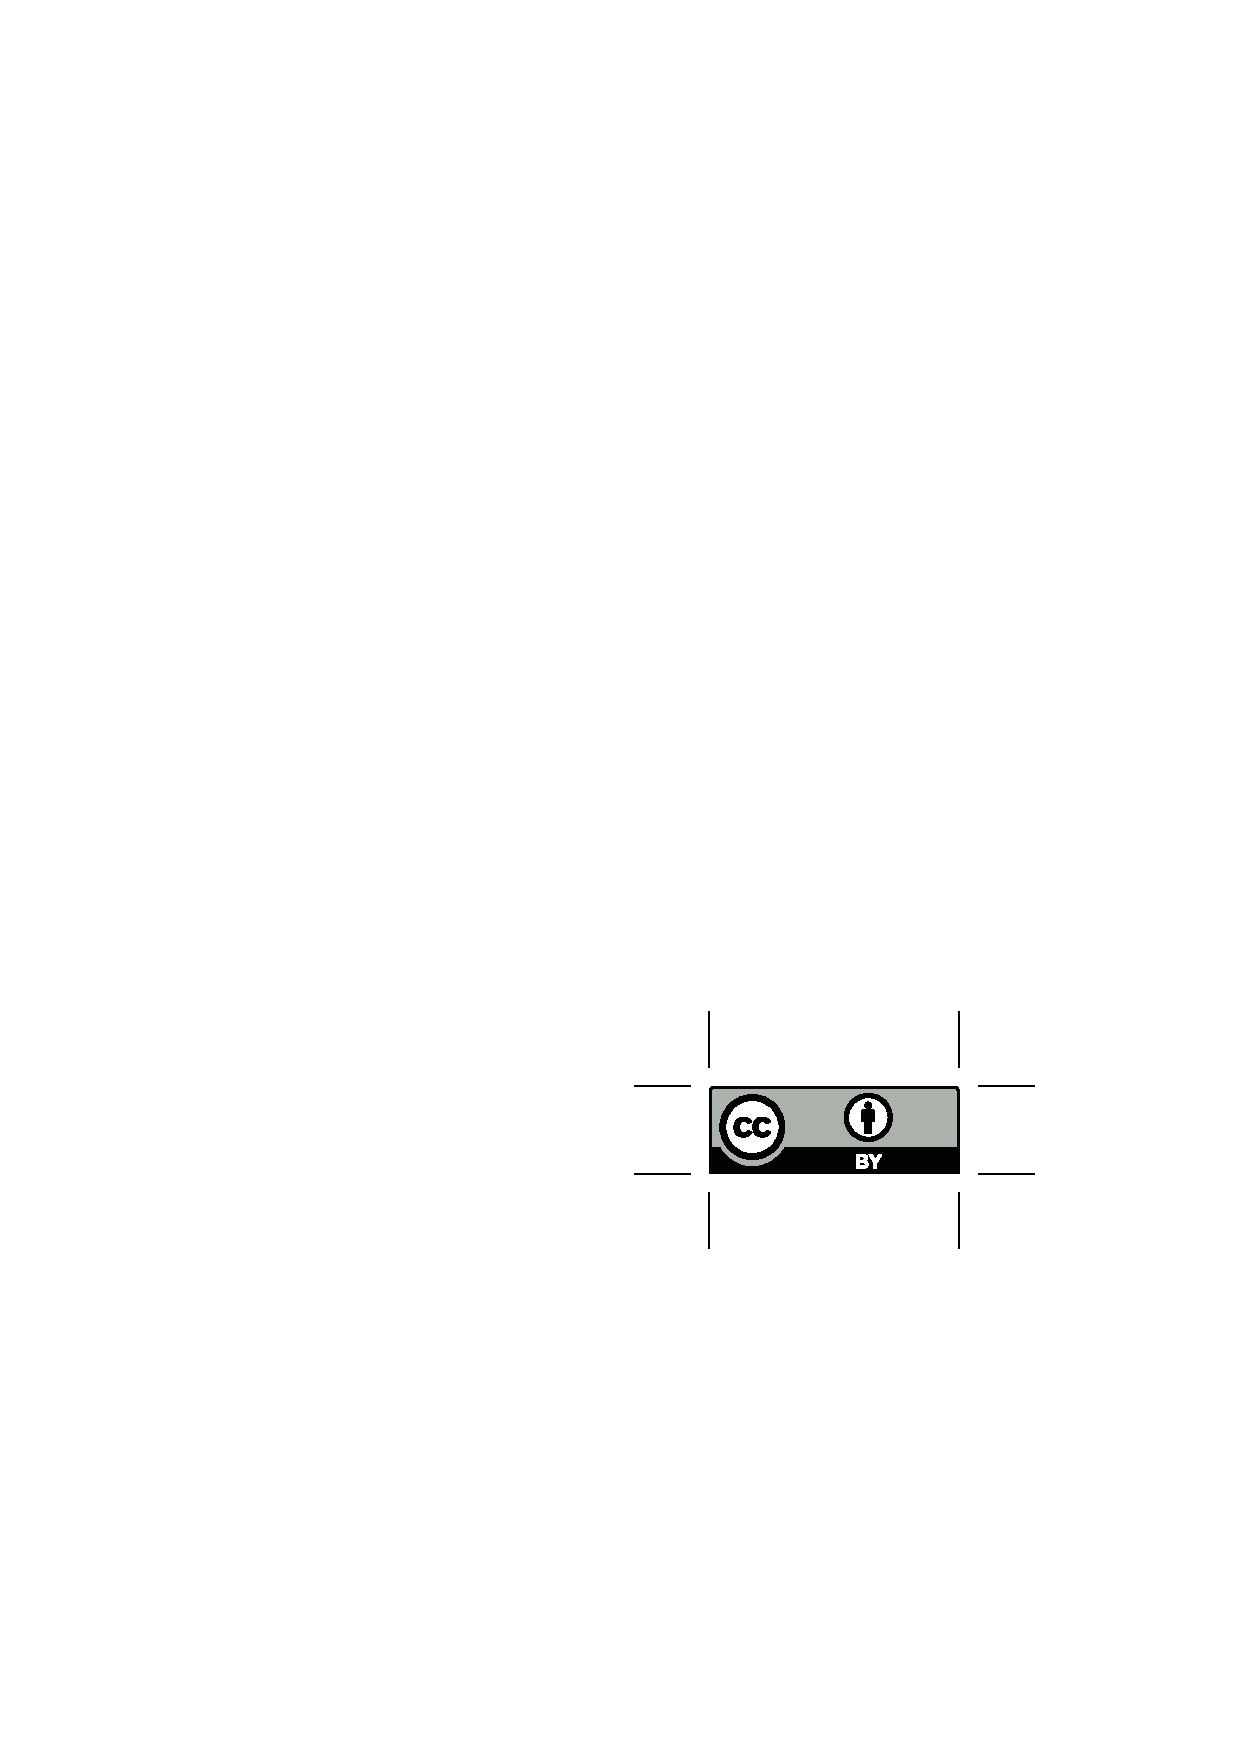
\includegraphics[width=\hsize]{dccpaper-by}}%
      \end{minipage}
      \par
      \bigskip
      \makebox[0pt][l]{\parbox{0.4\hsize}{%
        \ifx\undefined\dccp@titlefoot@bib\else\dccp@titlefoot@bib\fi
      }}\hfill
      \makebox[0pt][c]{\normalsize\thepage}\hfill
      \makebox[0pt][r]{\parbox{0.4\hsize}{%
        \raggedleft\ifx\undefined\dccp@titlefoot@doi\else\dccp@titlefoot@doi\fi
      }}%
    \end{minipage}%
  }%
  \let\@evenfoot=\@oddfoot
  \let\TitleFoot=\@oddfoot
}
%    \end{macrocode}
% \end{macro}
% \end{macro}
% \end{macro}
%
% We set the normal page style to \val{title} here so that \cs{TitleHead} and
% \cs{TitleFoot} are defined, but we will override it with the \val{dccpaper}
% page style later.
%
%    \begin{macrocode}
\pagestyle{title}
%    \end{macrocode}
%
% The first page should use the \val{title} page style, however.
%
%    \begin{macrocode}
\AtBeginDocument{\thispagestyle{title}}

%    \end{macrocode}
%
% \begin{macro}{ps@dccpaper}
% \begin{macro}{NormalHead}
% \begin{macro}{NormalFoot}
% Here are the normal headers and footers (i.e.\ the \val{dccpaper} page
% style). We save them to \cs{NormalHead} and \cs{NormalFoot}, again so we can
% measure them.
%
%    \begin{macrocode}
\def\ps@dccpaper{%
  \def\@oddhead{%
    \begin{minipage}{\textwidth}\frenchspacing
      {%
        \fontsize{9pt}{11pt}\selectfont
        \ifx\undefined\dccp@normhead@doi\else\dccp@normhead@doi\fi
      }\hfill
      {\MainAuthor}\space\space\space
      \textcolor{struct}{\textbar}\space\space\space
      \thepage\par
      \vskip6pt\color{struct}{\hrule height 1bp}\par
    \end{minipage}
  }%
  \def\@evenhead{%
    \begin{minipage}{\textwidth}
      \thepage\space\space\space
      \textcolor{struct}{\textbar}\space\space\space
      {\HeadTitle}\hfill
      {%
        \fontsize{9pt}{11pt}\selectfont
        \ifx\undefined\dccp@normhead@doi\else\dccp@normhead@doi\fi
      }\par
      \vskip6pt\color{struct}{\hrule height 1bp}\par
    \end{minipage}
  }%
  \let\NormalHead=\@oddhead
  \def\@oddfoot{\begin{minipage}[b]{\textwidth}
    \centering\ifdefstring{\dccp@variant}{baskerville}{\sffamily}{\bfseries}%
    \normalsize\color{struct}
    \ifx\dccp@type\dccp@editorial
      \dccp@publ@long
    \else
      \dccp@publ@short\space\space\textbar\space\space\emph{\dccp@type}%
    \fi
    \par
  \end{minipage}}%
  \let\@evenfoot=\@oddfoot
  \let\NormalFoot=\@oddfoot
}
\pagestyle{dccpaper}

%    \end{macrocode}
% \end{macro}
% \end{macro}
% \end{macro}
%
% \begin{macro}{dccp@firstpagehead}
% \begin{macro}{dccp@firstpagefoot}
% \begin{macro}{dccp@restpagehead}
% \begin{macro}{dccp@restpagefoot}
% We need to wait until the author has supplied the necessary information before
% we can do our measuring and set the remainder of the geometry, so we do it at
% the end of the preamble. First we put our saved macros into boxes we can
% measure (i.e.\ \cs{dccp@firstpagehead}, \cs{dccp@firstpagefoot},
% \cs{dccp@restpagehead}, \cs{dccp@restpagefoot}).
%
%    \begin{macrocode}
\AtEndPreamble{
  \newsavebox{\dccp@firstpagehead}
  \sbox\dccp@firstpagehead{\normalfont\TitleHead}
  \newsavebox{\dccp@firstpagefoot}
  \sbox\dccp@firstpagefoot{\normalfont
    \def\email#1{#1}\def\url#1{#1}\def\href#1#2{#2}\TitleFoot}
  \newsavebox{\dccp@restpagehead}
  \sbox\dccp@restpagehead{\normalfont\NormalHead}
  \newsavebox{\dccp@restpagefoot}
  \sbox\dccp@restpagefoot{\normalfont\NormalFoot}
%    \end{macrocode}
% \end{macro}
% \end{macro}
% \end{macro}
% \end{macro}
%
% We can now set the geometry of the title page\dots
%
%    \begin{macrocode}
  \setlength{\headheight}{\ht\dccp@firstpagehead + \dp\dccp@firstpagehead}
  \setlength{\footskip}{%
    2\baselineskip + \ht\dccp@firstpagefoot + \dp\dccp@firstpagefoot
  }
  \setlength{\textheight}{%
    \paperheight
    - 30mm % 15mm top and bottom
    - \headheight
    - \headsep
    - \footskip
  }
%    \end{macrocode}
%
% \begin{macro}{dccp@resetgeometry}
% {\dots}and provide a macro that will reset the geometry for the remaining
% pages.
%
%    \begin{macrocode}
  \def\dccp@resetgeometry{%
    \setlength{\headheight}{\ht\dccp@restpagehead + \dp\dccp@restpagehead}
    \global\headheight=\headheight
    \setlength{\footskip}{%
      2\baselineskip + \ht\dccp@restpagefoot
    }
    \global\footskip=\footskip
    \setlength{\textheight}{%
      \paperheight
      - 30mm % 15mm top and bottom
      - \headheight
      - \headsep
      - \footskip
    }
    \FixTextHeight
    \global\textheight=\textheight
  }
}

%    \end{macrocode}
% \end{macro}
%
% \begin{macro}{maketitle}
% The \cs{maketitle} command is redefined to the correct formatting. At the end it
% sets a hook that will reset the geometry when the first page is shipped out,
% i.e.\ with effect from the second page. It is here rather than at the end of
% the abstract in case the abstract itself spills over to the second page.
%
%    \begin{macrocode}
\RequirePackage{atbegshi}
\renewcommand{\maketitle}{%
  \null\nobreak\vspace*{-0.528\baselineskip}%
  \begingroup
    \centering
    {\Large\ifdefstring{\dccp@variant}{baskerville}{\bfseries}{}\thetitle\par}
    \vspace{0.7\baselineskip}
    \AuthorBlock\par
    \vspace{1.7\baselineskip}
  \endgroup
  \AtBeginShipoutNext{\dccp@resetgeometry}%
}

%    \end{macrocode}
% \end{macro}
%
% \begin{environment}{widequote}
% \begin{macro}{afterabstract}
% \begin{environment}{abstract}
% The \env{abstract} environment is redefined in terms of an environment
% \env{widequote}, which mimics the \env{quote} environment, but is a bit
% wider. We also provide a hook, \cs{afterabstract}, so that if some annotation
% needs to be appended to the title page after the abstract, we can do that.
%
%    \begin{macrocode}
\newenvironment{widequote}{%
  \list{}{%
    \setlength{\rightmargin}{2\parindent}%
    \setlength{\leftmargin}{2\parindent}%
  }%
  \flushleftright\item[]%
}{%
    \endlist
}
\def\afterabstract{}
\renewenvironment{abstract}{%
  \vskip1em%
  \begin{center}%
    {\bfseries\abstractname\vspace{-.5em}\vspace{\z@}}%
  \end{center}%
  \widequote\footnotesize
}{%
  \endwidequote\afterabstract\newpage
}

%    \end{macrocode}
% \end{environment}
% \end{macro}
% \end{environment}
%
% We use the \pkg{titlesec} package to give headings the correct formatting.
% The settings below try to space out headings so they occupy an integer number
% of normal lines (an attempt at grid typesetting). They are a little
% complicated because we want it to work even if the heading appears at the top
% of the page.
%
%    \begin{macrocode}
\RequirePackage{titlesec}
\titlespacing*{\section}{0pt}{0pt}{\baselineskip}
\titlespacing*{\subsection}{0pt}{0pt}{0.6\baselineskip}
\titlespacing{\subsubsection}{\parindent}{\baselineskip}{0pt}
\titlespacing{\paragraph}{\parindent}{\baselineskip}{0pt}
\titlespacing{\subparagraph}{\parindent}{\baselineskip}{0pt}
%    \end{macrocode}
%
% \begin{macro}{dccp@old@ep}
% An unfortunate side effect of spacing headings like this is that if a
% \cs{subsection} immediately follows a \cs{section} it forms an unsightly gap. To
% remedy this, we count how many paragraphs there have been since the last
% \cs{section}. Note that as we do not normally number the sections, an automatic
% reset of the |sectionpars| counter within the |section| counter won't work.
%
%    \begin{macrocode}
\newcounter{sectionpars}
\let\dccp@old@ep\everypar
\newtoks\everypar
\dccp@old@ep{\the\everypar\stepcounter{sectionpars}}
%    \end{macrocode}
% \end{macro}
%
% We need to manually reset |sectionpars| when \cs{section} is called. Also,
% the normal font size is 12pt/14.5pt, while \cs{Large} is 17pt/22pt;
% so the \cs{Large} line height = 1.5172 $\times$ normal line height. Nevertheless
% it seems to work better if we let the heading eat 0.528\cs{baselineskip} into
% the 2\cs{baselineskip} of padding above it.
%
%    \begin{macrocode}
\titleformat{\section}
  [block]
  {%
    \vspace{2\baselineskip}%
    \nobreak
    \vspace*{-0.528\baselineskip}%
    \setcounter{sectionpars}{0}%
    \filcenter\normalfont\Large\bfseries
  }
  {\thesection}
  {1em}
  {}
%    \end{macrocode}
%
% The others use a \cs{normalsize} font so that makes life easier. The format
% for \cs{subsection} command includes conditional spacing: if the |sectionpars|
% counter equals 2, this means the heading immediately follows a \cs{section}, so
% less white space is needed.
%
%    \begin{macrocode}
\titleformat{\subsection}
  {%
    \ifnum\thesectionpars>2%
      \vspace{2\baselineskip}%
    \else
      \vspace{\baselineskip}%
    \fi\nobreak
    \vspace*{-0.6\baselineskip}%
    \normalfont\normalsize\bfseries
  }
  {\thesubsection}
  {1em}
  {}
\titleformat{\subsubsection}
  [block]
  {\normalfont\normalsize\bfseries}
  {\thesubsubsection}
  {1em}
  {}
\titleformat{\paragraph}
  [block]
  {\normalfont\normalsize\bfseries\itshape}
  {\thesubsubsection}
  {1em}
  {}
\titleformat{\subparagraph}
  [block]
  {\normalfont\normalsize\itshape}
  {\thesubsubsection}
  {1em}
  {}
%    \end{macrocode}
%
% DCC papers do not typically number their sections.
%
%    \begin{macrocode}
\setcounter{secnumdepth}{0}

%    \end{macrocode}
%
% To help with the display of tables we load the \pkg{array} and
% \pkg{booktabs} packages. As we don't like lines between rows in the table
% body, we stretch them out a bit so that white space does the job instead.
%
%    \begin{macrocode}
\RequirePackage{array,booktabs}
\renewcommand{\arraystretch}{1.25}

%    \end{macrocode}
%
% We use the \pkg{caption} package to give captions the right format.
%
%    \begin{macrocode}
\RequirePackage
  [ format=hang
  , labelsep=period
  , font=small
  , labelfont=bf
  , figureposition=bottom
  , tableposition=top
  ]{caption}

%    \end{macrocode}
%
% \begin{macro}{footnotelayout}
% Footnotes should be set right up against the left margin. They should be
% set hung and in the same half-ragged style as the main text. They should also,
% for neatness, be at the bottom of the page regardless of how short it is. The
% \pkg{footmisc} package helps here.
%
%    \begin{macrocode}
\RequirePackage[hang,bottom]{footmisc}
\settowidth{\footnotemargin}{\footnotesize\textsuperscript{99}\space}
\renewcommand{\footnotelayout}{\raggedyright}
%    \end{macrocode}
% \end{macro}
%
% \begin{macro}{dccp@footnote}
% \begin{macro}{dccp@next@token}
% \begin{macro}{dccp@supercomma}
% \begin{macro}{dccp@check@for@footnote}
% Also, if multiple footnotes are set at once, the markers should be separated
% with superscript commas. The \pkg{footmisc} package should help here but
% its solution is clobbered by \pkg{hyperref}. So after a footnote is set,
% we check to see if the next token is also a footnote, and if so, slip a comma
% in before it.\footnote{This solution was provided at
% \url{http://tex.stackexchange.com/q/40072}} This tweak needs to be done late,
% \cs{AtBeginDocument}. Note that the \pkg{newtx} superior figures are a bit
% lower than normal superscript text.
%
%    \begin{macrocode}
\AtBeginDocument{
  \let\dccp@footnote\footnote
  \def\dccp@next@token{\relax}%
  \def\dccp@supercomma{\textsuperscript{,}}%
  \IfFileExists{newtxtext.sty}%
    {\def\dccp@supercomma{\raisebox{-0.2ex}{\textsuperscript{,}}}}%
    {}

  \newcommand\dccp@check@for@footnote{%
    \ifx\footnote\dccp@next@token
      \dccp@supercomma
    \fi
  }

  \renewcommand\footnote[1]{%
    \dccp@footnote{#1}%
    \futurelet\dccp@next@token\dccp@check@for@footnote
  }
}

%    \end{macrocode}
% \end{macro}
% \end{macro}
% \end{macro}
% \end{macro}
%
% By default lists are quite loose. These settings help to tighten them.
%
%    \begin{macrocode}
\topsep = \z@
\partopsep = \z@
\appto{\enumerate}{\itemsep = 0.5ex plus 0.25ex minus 0.25ex}
\appto{\itemize}{\itemsep = 0.5ex plus 0.25ex minus 0.25ex}

%    \end{macrocode}
%
% A DCC paper should either be using \pkg{biblatex} or \pkg{apacite} for
% references.
%
% If \pkg{biblatex} is used, we need to ensure that the reference list
% heading is a normal section rather than a starred one so it appears in the
% PDF bookmarks.
%
%    \begin{macrocode}
\AtBeginDocument{
  \@ifpackageloaded{biblatex}{%
    \defbibheading{bibliography}[\refname]{\section{#1}}%
%    \end{macrocode}
%
% We also move the ‘doi:’ portion of a DOI inside the hyperlink.
%
%    \begin{macrocode}
    \DeclareFieldFormat{doi}{%
      \ifhyperref{%
        \href{https://doi.org/#1}{\nolinkurl{doi:#1}}%
      }{%
        \nolinkurl{doi:#1}%
      }%
    }
  }{%
%    \end{macrocode}
%
% If \pkg{apacite} is used, there are a few other adaptations we need to
% make.
%
%    \begin{macrocode}
    \@ifpackageloaded{apacite}{%
%    \end{macrocode}
%
% \begin{macro}{@ifauthorsunequalc@de}
% With \pkg{hyperref} loaded, \pkg{apacite} makes the whole of a citation
% a link to the reference list item. We patch \cs{@ifauthorsunequalc@de} so only
% the year portion gets linked.
%
%    \begin{macrocode}
      \def\@ifauthorsunequalc@de#1{%
        \if@F@cite
          \@F@citefalse
        \else
          \if@Y@cite
              {\@BAY}%
          \fi
          {\@BBC}%
        \fi
        \edef\@cite@undefined{?}%
        \def\BBA{\@BBA}%
        \if@A@cite
          %%\hyper@natlinkstart{#1}% We remove this line...
          {\csname b@\@citeb\APAC@extra@b@citeb\endcsname}%
          %%\hyper@natlinkend% ...and this one.
          \if@Y@cite
              {\@BBAY}%
          \fi
        \fi
        \if@Y@cite
          \hyper@natlinkstart{#1}%
          {\csname Y@\@citeb\APAC@extra@b@citeb\endcsname}%
          \hyper@natlinkend
        \fi
        \let\BBA\relax
      }
%    \end{macrocode}
% \end{macro}
%
% The Spanish language support file defines a different version of
% \cs{@ifauthorsunequalc@de}, which might override the patch we have just
% introduced. So we employ the same test that \pkg{apacite} uses when
% deciding whether to load that file; if successful, we patch the Spanish
% version. Note that as \pkg{apacite} loads language support files
% \cs{AtBeginDocument}, we have to do our thing after that, \cs{AfterEndPreamble}.
%
% (Note that as we set the language to British English earlier, this should
% never be needed, but we try to be resilient to tinkering!)
%
%    \begin{macrocode}
      \AfterEndPreamble{%
        \@ifundefined{iflanguage}{%
          \relax
        }{%
          \edef\APAC@tmp{nohyphenation}%
          \ifx\languagename\APAC@tmp
          \else
            \edef\APAC@tmp{spanish}%
            \ifx\languagename\APAC@tmp
              \def\@ifauthorsunequalc@de#1{%
                \if@F@cite
                  \@F@citefalse
                \else
                  \if@Y@cite
                      {\@BAY}%
                  \fi
                  {\@BBC}%
                \fi
                \edef\@cite@undefined{?}%
                \def\BBA{\@BBA}%
                \@ifundefined{spanishe@\@citeb\APAC@extra@b@citeb}%
                  {}% skip
                  {{% Use `e' instead of `y' in Spanish
                  \global\let\oldBBA\BBA
                  \global\def\BBA{e\global\let\BBA\oldBBA}%
                  }}%
                \if@A@cite
                  %%\hyper@natlinkstart{#1}% We remove this line...
                  {\csname b@\@citeb\APAC@extra@b@citeb\endcsname}%
                  %%\hyper@natlinkend% ...and this one.
                  \if@Y@cite
                      {\@BBAY}%
                  \fi
                \fi
                \if@Y@cite
                  \hyper@natlinkstart{#1}%
                  {\csname Y@\@citeb\APAC@extra@b@citeb\endcsname}%
                  \hyper@natlinkend
                \fi
                \let\BBA\relax
              }%
            \fi
          \fi
        }%
%    \end{macrocode}
%
% Another thing \pkg{apacite} does \cs{AtBeginDocument} is set the URL style
% to monospaced. So we reset it back to normal roman type \cs{AfterEndPreamble}.
%
%    \begin{macrocode}
        \urlstyle{APACrm}
       }%
%    \end{macrocode}
%
% \begin{macro}{doi}
% \begin{macro}{doiprefix}
% We pre-empt \pkg{apacite}'s \cs{providecommand} of \cs{doi} with our own
% definition that includes the `doi' URI scheme label in the link, remembering
% to remove the one inserted by \cs{doiprefix}.
%
%    \begin{macrocode}
      \newcommand{\doi}[1]{\href{https://doi.org/#1}{\nolinkurl{doi:#1}}}%
      \renewcommand{\doiprefix}{\unskip}%
    }{}%
  }%
%    \end{macrocode}
% \end{macro}
% \end{macro}
%
% \begin{macro}{bibitemsep}
% Both \pkg{biblatex} and \pkg{apacite} use \cs{bibitemsep} for the space
% between bibliography items. Just in case they haven't been loaded, though, we
% protect our setting of that length with an \cs{ifx} test.
%
%    \begin{macrocode}
  \ifx\undefined\bibitemsep
  \else
    \setlength{\bibitemsep}{1em plus 1ex minus 1ex}%
  \fi
}
%    \end{macrocode}
% \end{macro}
%
% As mentioned above, if \pkg{apacite} is used, we can use a package option
% to ensure that the reference list heading appears in the PDF bookmarks.
%
%    \begin{macrocode}
\PassOptionsToPackage{numberedbib}{apacite}

%    \end{macrocode}
%
% We, of course, use \pkg{hyperref} for enhancing the PDF with working links,
% bookmarks, metadata, etc.
%
%    \begin{macrocode}
\RequirePackage
  [ colorlinks=true
  , linkcolor=black
  , anchorcolor=black
  , citecolor=links
  , filecolor=black
  , menucolor=black
  , runcolor=black
  , urlcolor=links
  ]{hyperref}
%    \end{macrocode}
%
% Links should be in roman type, not monospaced.
%
%    \begin{macrocode}
\urlstyle{rm}
%    \end{macrocode}
%
% \begin{macro}{email}
% We provide an \cs{email} command for displaying the email address of the
% corresponding author.
%
%    \begin{macrocode}
\newcommand*{\email}[1]{\href{mailto:#1}{#1}}
%    \end{macrocode}
% \end{macro}
%
% Once the user has had a chance to provide the metadata, we can add it to the
% PDF metadata.
%
%    \begin{macrocode}
\AtBeginDocument{%
  \hypersetup
    { pdftitle={\thetitle}
    , pdfauthor={\dccp@author}
    , pdfsubject={\dccp@subject}
    }
%    \end{macrocode}
%
% The APA has its own style for line breaks in URLs. The \pkg{apacite}
% package provides the code for this, but in case \pkg{biblatex} is used
% instead, we repeat the settings (from 2013/07/21 v6.03) here.
%
%    \begin{macrocode}
  \@ifundefined{Url@force@Tilde}{\def\Url@force@Tilde{\relax}}{}%
  \def\url@apa@dot{\mathchar"2E }%
  \def\url@apa@comma{\mathchar"2C }%
  \def\url@apa@questionmark{\mathchar"3F }%
  \def\url@apa@exclamation{\mathchar"21 }%
  \def\url@apa@hyphen{\mathchar"2D }%
  \def\url@apa@underscore{\_}%
  \def\UrlBreaks{\do\@\do\\\do\|\do\;\do\>\do\]\do\)\do\'\do+\do\=\do\#}%
  \def\UrlBigBreaks{\do\/\do\:\do@url@hyp}%
  \def\UrlNoBreaks{\do\(\do\[\do\{\do\<}% \)}
  \def\UrlOrds{\do\*\do\~\do\'\do\"}%
  \def\UrlSpecials{%
    \do\.{\mathbin{}\url@apa@dot }%
    \do\,{\mathbin{}\url@apa@comma }%
    \do\-{\mathbin{}\url@apa@hyphen }%
    \do\?{\mathbin{}\url@apa@questionmark }%
    \do\!{\mathbin{}\url@apa@exclamation }%
    \do\_{\mathbin{}\url@apa@underscore }%
    \do\ {\Url@space}\do\%{\Url@percent}\do\^^M{\Url@space}%
    \Url@force@Tilde}%
  \def\Url@OTnonTT{\do\<{\langle}\do\>{\mathbin{\rangle}}\do
    \_{\mathbin{}\_}\do\|{\mid}\do\{{\lbrace}\do\}{\mathbin{\rbrace}}\do
    \\{\mathbin{\backslash}}\UrlTildeSpecial}
}

%    \end{macrocode}
%
% We now embed the Creative Commons licence information in the PDF using an XMP
% packet. To do this, we employ the same technique as Scott Pakin's
% \pkg{hyperxmp} (2014/01/02 v2.4). In order to avoid avoid a bug whereby
% Adobe Acrobat confuses the XMP author information and the regular author
% information, though, we \emph{only} embed the licence information.
%
% We need to make sure that any characters to appear verbatim in the XMP packet
% are treated as ordinary characters and not active ones. The likely active
% characters are symbols and punctuation, so should be treated as `other'
% (category 12).
%
%    \begin{macrocode}
\begingroup
\catcode`\"=12
\catcode`\&=12
\catcode`\#=12
\catcode`\<=12
\catcode`\>=12
\catcode`\_=12
%    \end{macrocode}
%
% We construct the XMP packet as the document begins.
%
%    \begin{macrocode}
\AtBeginDocument{%
%    \end{macrocode}
%
% \begin{macro}{sp}
% For convenience we define \cs{sp} to be a level of indent, translating to three
% spaces.
%
%    \begin{macrocode}
  \def\sp{\space\space\space}
%    \end{macrocode}
% \end{macro}
%
% The text of the XMP packet is recorded in \cs{cc@xmp@packet}. We use |^^J| to
% break lines.
%
%    \begin{macrocode}
  \long\gdef\cc@xmp@packet{%
<?xpacket begin='' id=''?>^^J%
<x:xmpmeta xmlns:x='adobe:ns:meta/'>^^J%
<rdf:RDF xmlns:rdf='http://www.w3.org/1999/02/22-rdf-syntax-ns#'>^^J%
\sp<rdf:Description rdf:about=''^^J%
\sp\sp xmlns:xapRights='http://ns.adobe.com/xap/1.0/rights/'>^^J%
\sp\sp<xapRights:Marked>True</xapRights:Marked>^^J%
\sp</rdf:Description>^^J%
\sp<rdf:Description rdf:about=''^^J%
\sp\sp xmlns:dc='http://purl.org/dc/elements/1.1/'>^^J%
\sp\sp<dc:rights>^^J%
\sp\sp\sp<rdf:Alt>^^J%
\sp\sp\sp\sp<rdf:li xml:lang='x-default'>This work is licensed under a Creative Commons Attribution 4.0 International Licence.</rdf:li>^^J%
\sp\sp\sp</rdf:Alt>^^J%
\sp\sp</dc:rights>^^J%
\sp</rdf:Description>^^J%
\sp<rdf:Description rdf:about=''^^J%
\sp\sp xmlns:cc='http://creativecommons.org/ns#'>^^J%
\sp\sp<cc:license rdf:resource='http://creativecommons.org/licenses/by/4.0/'/>^^J%
\sp</rdf:Description>^^J%
</rdf:RDF>^^J%
</x:xmpmeta>^^J%
<?xpacket end='r'?>^^J%
  }%
}
\endgroup
%    \end{macrocode}
%
% Different workflows require the XMP packet to be embedded in different ways.
%
% \begin{macro}{ccxmp@embed@packet@pdftex}
% Pdf\TeX\ can inject objects into PDFs natively.
%
%    \begin{macrocode}
\newcommand*{\ccxmp@embed@packet@pdftex}{%
  \bgroup
    \pdfcompresslevel=0
    \immediate\pdfobj stream attr {%
      /Type /Metadata
      /Subtype /XML
    }{\cc@xmp@packet}%
    \pdfcatalog {/Metadata \the\pdflastobj\space 0 R}%
  \egroup
}
%    \end{macrocode}
% \end{macro}
%
% \begin{macro}{ccxmp@embed@packet@pdfmark}
% The \cs{pdfmark} command defined by \pkg{hyperref} is respected by tools such
% as Dvipdf, Dvips, Dvipsone, etc.
%
%    \begin{macrocode}
\newcommand*{\ccxmp@embed@packet@pdfmark}{%
  \pdfmark{%
    pdfmark=/NamespacePush
  }%
  \pdfmark{%
    pdfmark=/OBJ,
    Raw={/_objdef \string{ccxmp@packet\string} /type /stream}%
  }%
  \pdfmark{%
    pdfmark=/PUT,
    Raw={\string{ccxmp@packet\string}
      2 dict begin
        /Type /Metadata def
        /Subtype /XML def
        currentdict
      end
    }%
  }%
  \pdfmark{%
    pdfmark=/PUT,
    Raw={\string{ccxmp@packet\string} (\cc@xmp@packet)}%
  }%
  \pdfmark{%
    pdfmark=/Metadata,
    Raw={\string{Catalog\string} \string{ccxmp@packet\string}}%
  }%
  \pdfmark{%
    pdfmark=/NamespacePop
  }%
}
%    \end{macrocode}
% \end{macro}
%
% Dvipdfm has its own \cs{special} command for inserting PDF objects, but
% it is a bit basic and requires advance knowledge of how long (in characters)
% the object is.
%
% \begin{macro}{ccxmp@count@spaces}
% The \cs{ccxmp@count@spaces} macro counts the number of spaces in its parameter
% through a process of iteration, adding this figure to \cs{@tempcnta}.
%
%    \begin{macrocode}
\def\ccxmp@count@spaces#1 {%
  \def\ccxmp@one@token{#1}%
  \ifx\ccxmp@one@token\@empty
    \advance\@tempcnta by -1
  \else
    \advance\@tempcnta by 1
    \expandafter\ccxmp@count@spaces
  \fi
}
%    \end{macrocode}
% \end{macro}
%
% \begin{macro}{ccxmp@count@non@spaces}
% The \cs{ccxmp@count@non@spaces} command counts the number of non-spaces in its
% argument through a process of iteration, adding this figure to \cs{@tempcnta}.
%
%    \begin{macrocode}
\newcommand*{\ccxmp@count@non@spaces}[1]{%
  \def\ccxmp@one@token{#1}%
  \ifx\ccxmp@one@token\@empty
  \else
    \advance\@tempcnta by 1
    \expandafter\ccxmp@count@non@spaces
  \fi
}
%    \end{macrocode}
% \end{macro}
%
% \begin{macro}{ccxmp@string@len}
% The \cs{ccxmp@string@len} command sets \cs{@tempcnta} to the number of characters
% (spaces + non-spaces) in its argument.
%
%    \begin{macrocode}
\newcommand*{\ccxmp@string@len}[1]{%
  \@tempcnta=0
  \expandafter\ccxmp@count@spaces#1 {} %
  \expandafter\ccxmp@count@non@spaces#1{}%
}
%    \end{macrocode}
% \end{macro}
%
% \begin{macro}{ccxmp@embed@packet@dvipdfm}
% So now, finally, is the command for embedding the packet using Dvipdfm.
%
%    \begin{macrocode}
\newcommand*{\ccxmp@embed@packet@dvipdfm}{%
  \ccxmp@string@len{\cc@xmp@packet}%
  \special{pdf: object @ccxmp@packet
    <<
      /Type /Metadata
      /Subtype /XML
      /Length \the\@tempcnta
    >>
    stream^^J\cc@xmp@packet endstream%
  }%
  \special{pdf: docview
    <<
      /Metadata @ccxmp@packet
    >>
  }%
}
%    \end{macrocode}
% \end{macro}
%
% \begin{macro}{ccxmp@embed@packet@xetex}
% \XeTeX\ creates PDFs with Xdvipdfmx, which supports a simpler \cs{special} for
% inserting objects that does not require us to count characters.
%
%    \begin{macrocode}
\newcommand*{\ccxmp@embed@packet@xetex}{%
  \special{pdf:stream @ccxmp@packet (\cc@xmp@packet)
    <<
      /Type /Metadata
      /Subtype /XML
    >>
  }%
  \special{pdf:put @catalog
    <<
      /Metadata @ccxmp@packet
    >>
  }%
}
%    \end{macrocode}
% \end{macro}
%
% We rely on \pkg{hyperref} to tell us how the PDF will be generated (after
% all, it may not be done in the current pass) and use the respective technique
% to embed the XMP packet.
%
%    \begin{macrocode}
\AtBeginDocument{%
  \begingroup
  \def\ccxmp@driver{hpdftex}%
  \ifx\ccxmp@driver\Hy@driver
    \ccxmp@embed@packet@pdftex
  \else
    \def\ccxmp@driver{hdvipdfm}%
    \ifx\ccxmp@driver\Hy@driver
      \ccxmp@embed@packet@dvipdfm
    \else
      \def\ccxmp@driver{hxetex}%
      \ifx\ccxmp@driver\Hy@driver
        \ccxmp@embed@packet@xetex
      \else
        \@ifundefined{pdfmark}{}{%
          \ccxmp@embed@packet@pdfmark
        }%
      \fi
    \fi
  \fi
  \endgroup
}
%    \end{macrocode}
% \iffalse
%</base>
% \fi
%\Finale
